\chapter{統計モデル}

\section{正規分布を含んだ統計モデル}
\begin{quote}
    \begin{enumerate}[(1)]
    \item 独立同分布
    \item その分布は、正規分布
    \item 正規分布の母数(平均と分散)はそれぞれ$\mu,\sigma^2$。
    \end{enumerate}
\end{quote}

\section{最尤推定量を使ったモデル}


\section{標本が統計モデルにより生成されたのかを判断する方法}%統計モデルの性質を使った方法}
%ここまでは、統計モデルの予測がデータと一致することを定量的に評価した。
ここでは、推測に適していないと判断する方法である、統計的仮説検定を紹介する。
この方法は、統計量の一つである統計検定量の統計モデル上での出現しやすさにより、モデルを評価する。
今回考えている統計モデル$M(\mu)$では、次の統計量$Z$が標準正規分布$N(0,1)$に従うことが、正規分布の再生性によってわかっている。
\if 0
 川久保統計学P.166
 \fi
$$
Z(\bar{X},\mu)=\frac{\sqrt{n}(\bar{X}-\mu)}{\sigma} \sim N(0,1)
$$
ここで$\bar{X}$は、統計モデル$M(\mu)$からサンプリングした標本の標本平均値(データの平均値ではない)、$\mu,\sigma$は統計モデルで設定した母数平均、母数分散。
$Z(\bar{X},\mu)$が$N(0,1)$に従うということから、$Z(\bar{X},\mu)$が$N(0,1)$における出現頻度が計算できる。

%![Z値の頻度]()
\begin{figure}
\begin{center}
    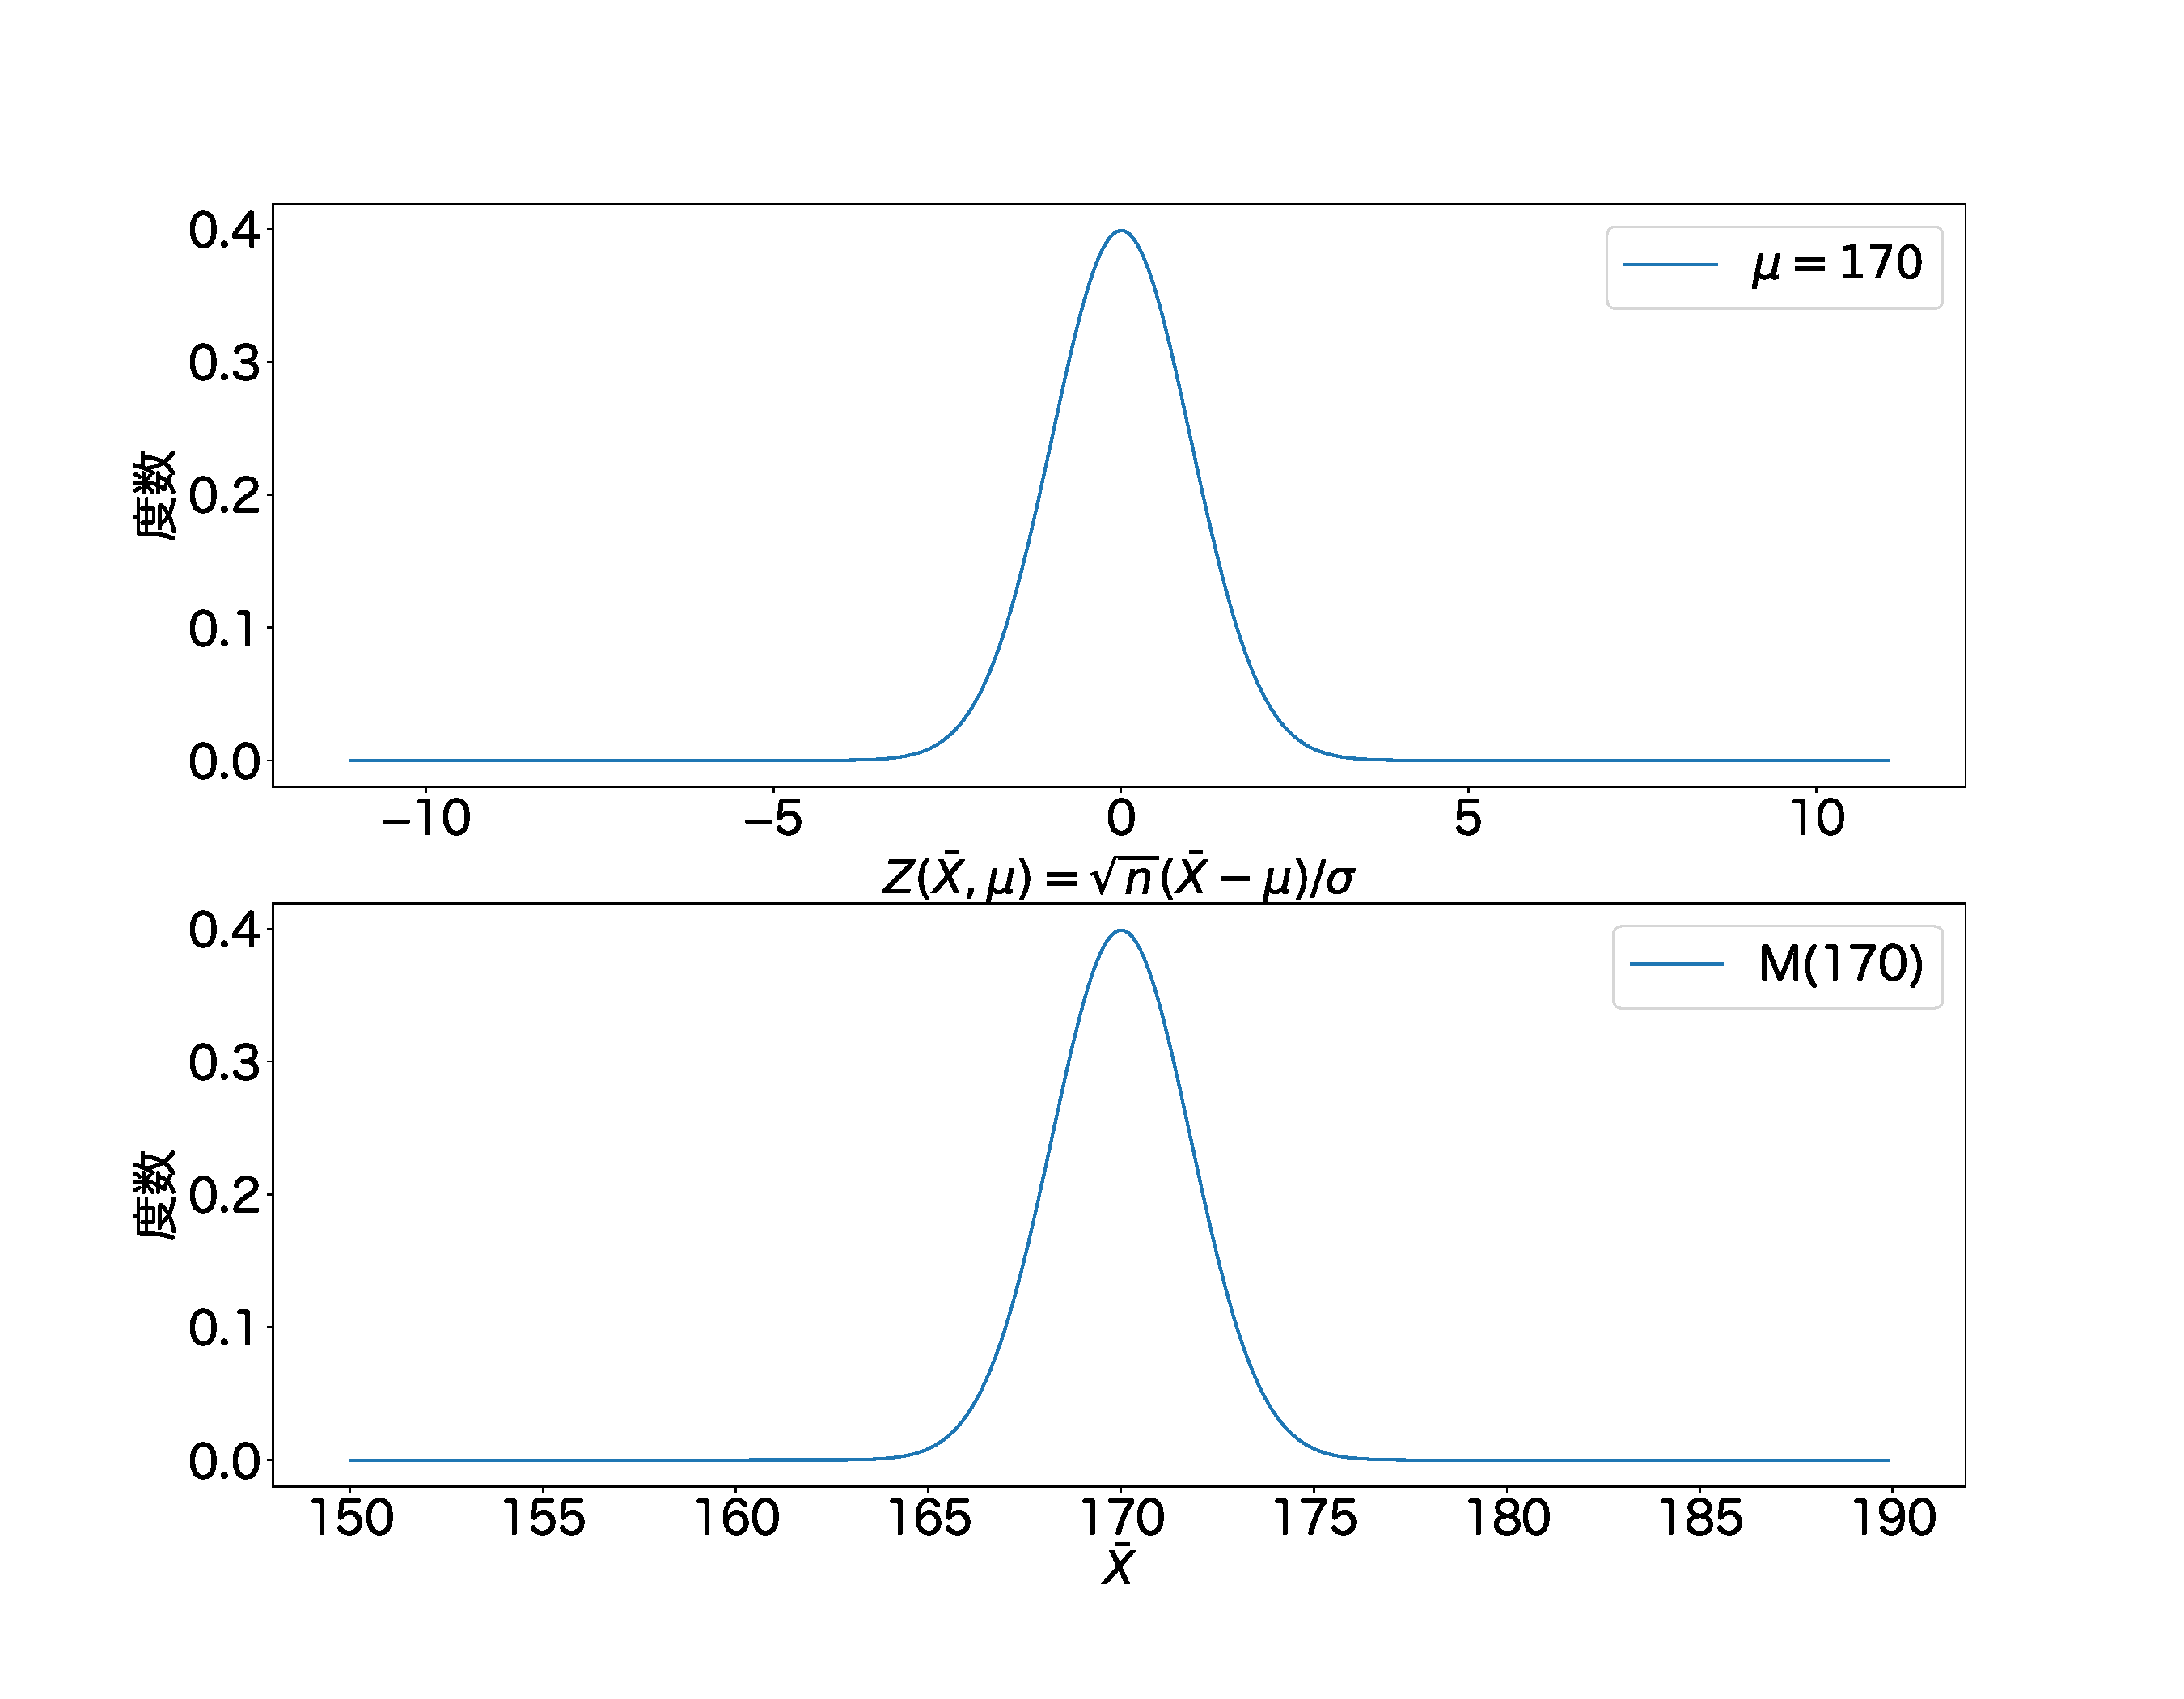
\includegraphics[width=15cm]{./image/03_/normal_Z_frequency.pdf}
    \label{fig:cm_standard_normal_distribution}
  \end{center}
\end{figure}

$Z$の出現頻度を$Z$または$\bar{X}$の値に応じて書いたものが図\ref{fig:cm_standard_normal_distribution}です。
$Z(\bar{X},\mu)$の$95\%$予測区間が次のように求められる。
$$
-z_{0.025}<Z(\bar{X},\mu)<z_{0.025}
$$
このの範囲で、サンプリングされた標本の統計量$Z(\bar{X},\mu)$が$95\%$の確率で得られる。
統計モデルを使った判断でよく出てくる確率として分野を問わず、$95\%$が使われる。
%この値には身長に関する経験を使わずに決定しています。


$Z(\bar{X},\mu)$を式変形することで、標本平均が$95\%$の確率で出現する区間が推定できる。式を変形する。
\begin{eqnarray*}
    & -z_{0.025} < Z(\bar{X},\mu)<z_{0.025} \\
\rightarrow & -z_{0.025} < \frac{\sqrt{n}(\bar{X}-\mu)}{\sigma}  <z_{0.025} \\
\rightarrow & \mu - z_{0.025} \frac{\sigma}{\sqrt{n}} < \bar{X} < \mu + z_{0.025} \frac{\sigma}{\sqrt{n}}
\end{eqnarray*}
この統計モデルからサンプリングした標本の標本平均$\bar{X}$が$95\%$の確率で見つかる範囲のことを$95\%$信頼区間という。
信頼区間の中に標本平均が含まれていることは、標本がモデルにり推測可能であることの証拠の一つになる。
ただし、証拠の一つであり、このことは実際には複合的に指標を見て判断する必要がある。
%$\bar{X}$が$95\%$信頼区間の中に入っていることは、この統計モデル

%信頼区間の中に統計量があれば、
%このことから、統計モデル$M(\mu)$でサンプリングしたときに、$95\%$の確率で、この範囲に平均値$\bar{X}$がえられます。

\subsection{サンプルサイズによる影響}
式を見てわかるように、サンプルサイズ$n$が大きくなれば、$\bar{x}$が入る範囲は狭くなる。
信頼区間がサンプルサイズに依存することを数値的に確認する。
図\ref{fig:confidence_interval_n}は、信頼区間が$N$に応じて変化する様子を図示している。


\begin{figure}
\begin{center}
    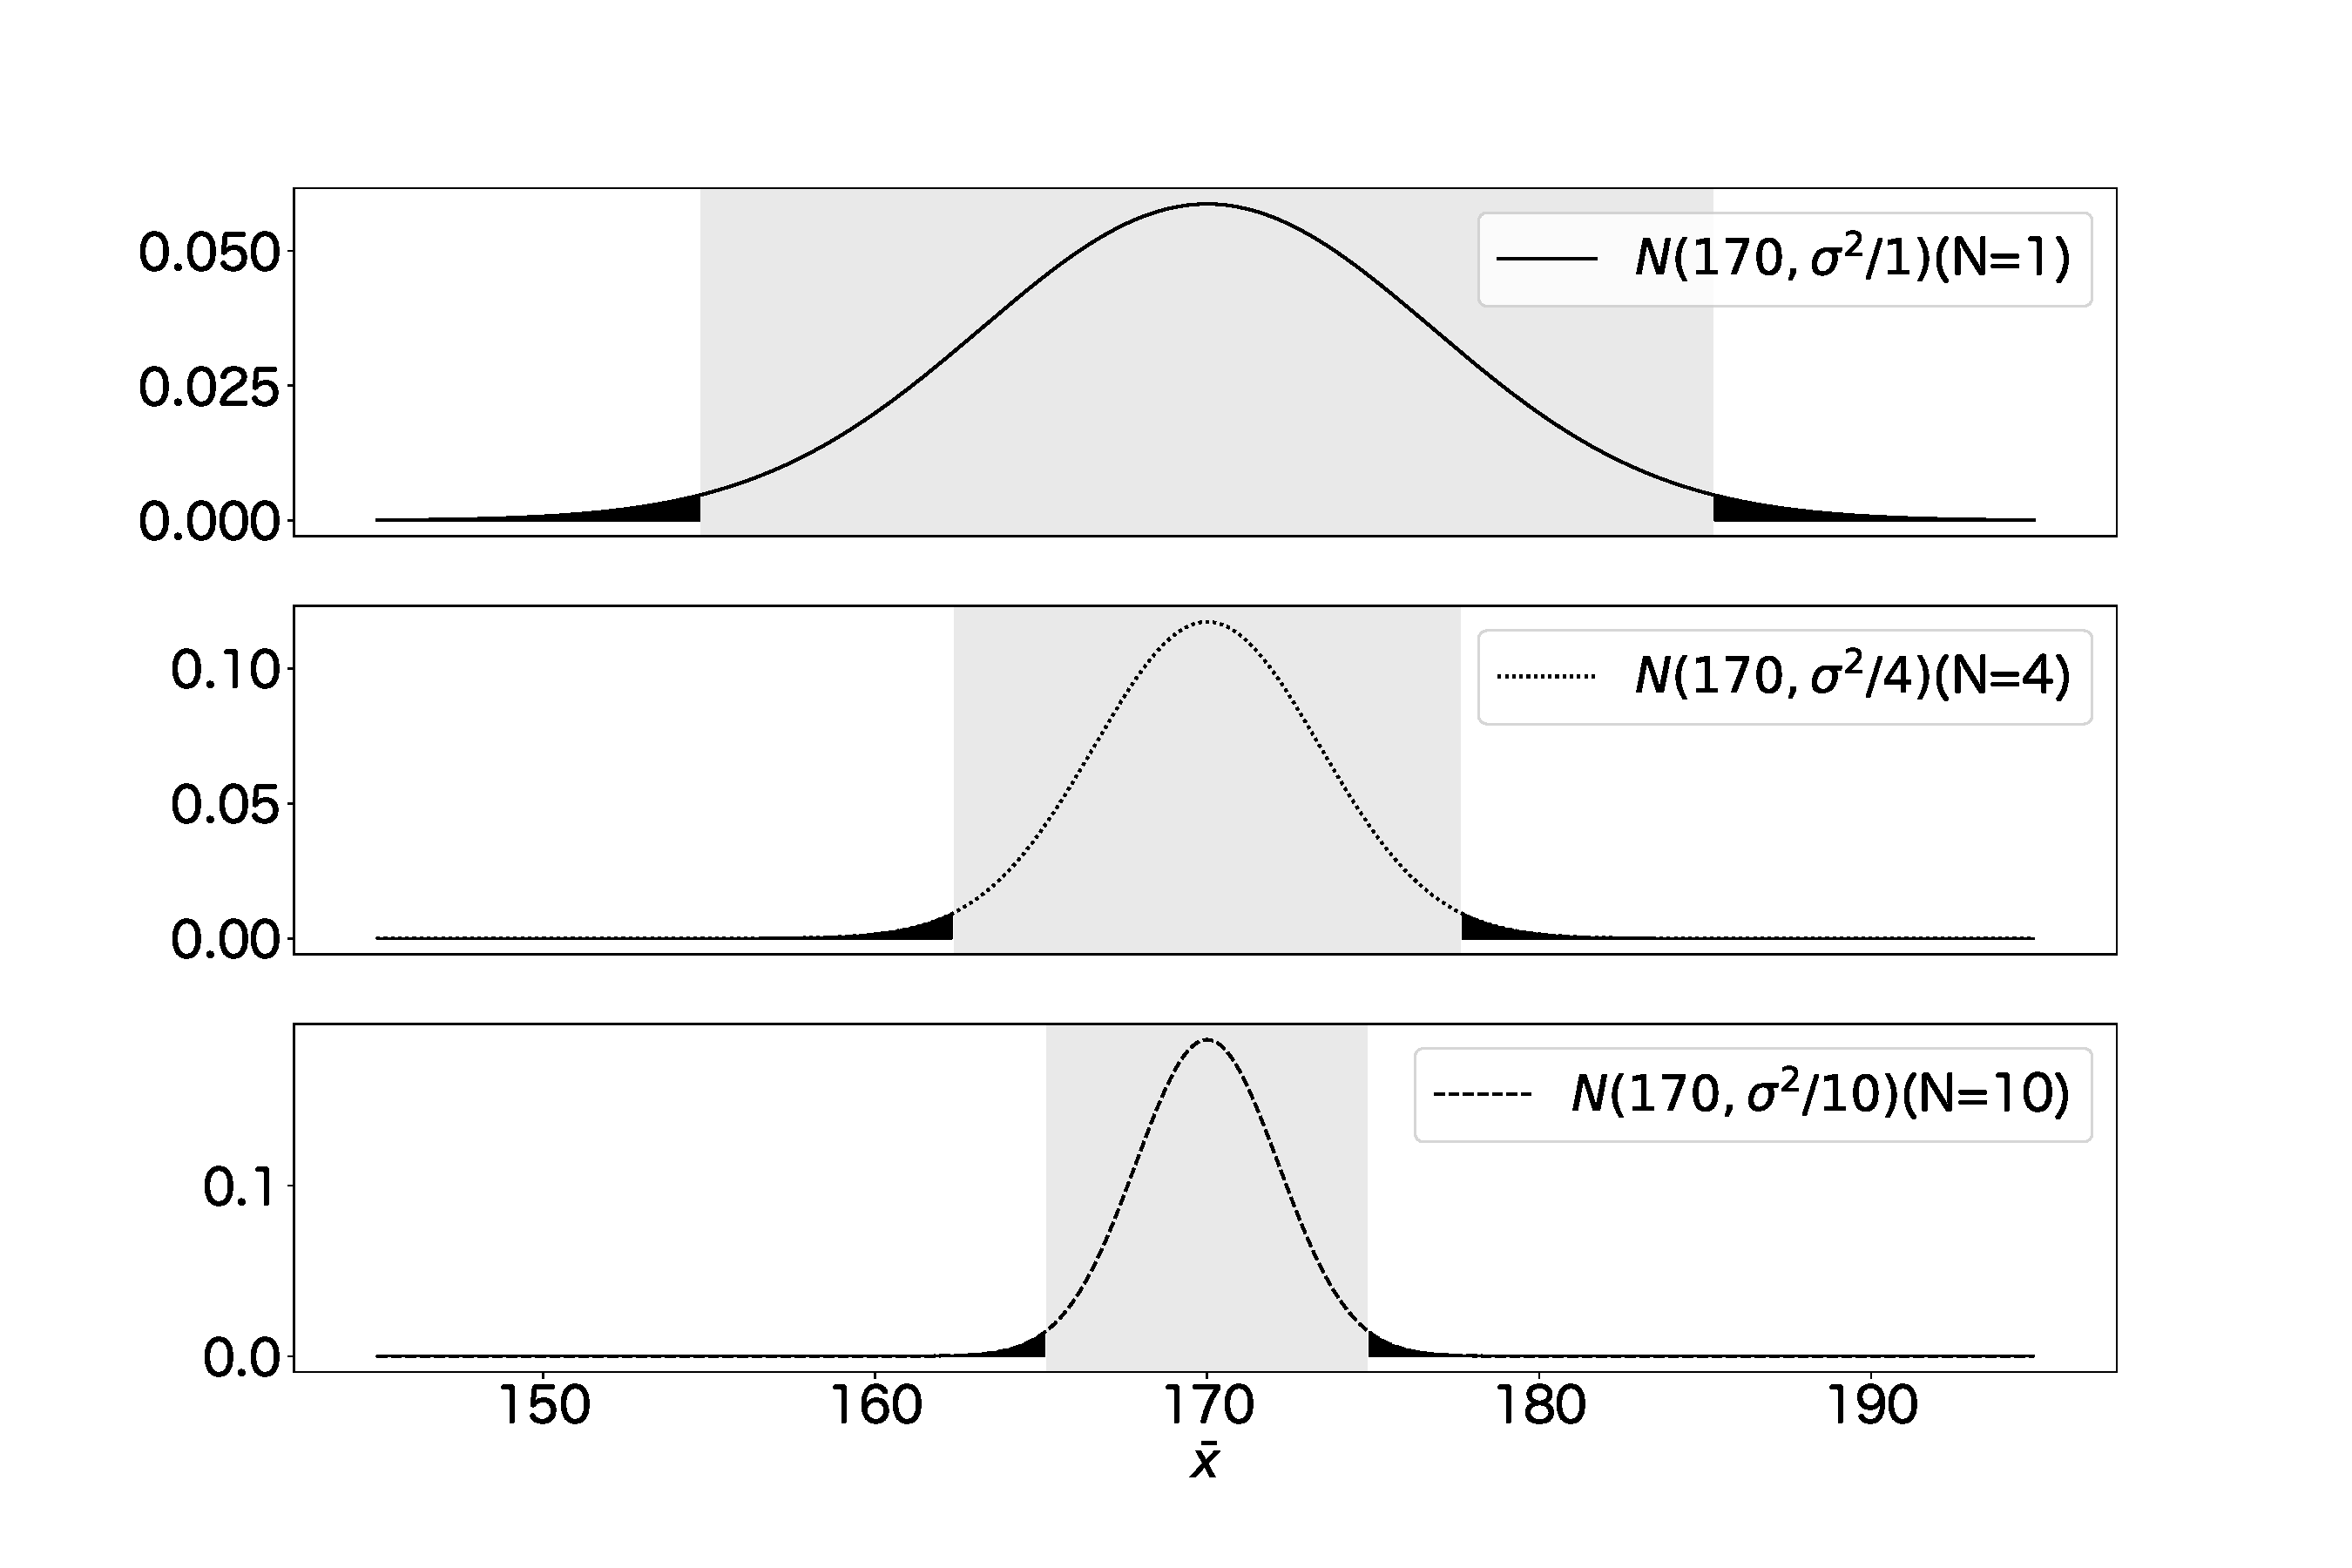
\includegraphics[width=15cm]{./image/03_/confidence_interval.pdf}
%    \caption{信頼区間}
    \caption{(A)$N=1$,(B)$N=4$,(C)$N=10$での信頼区間}
    \label{fig:confidence_interval_n}
  \end{center}
\end{figure}


\begin{framed}
    まとめ、
    \begin{itemize}
        \item 統計モデル$M(\mu)$によってサンプリングし、標本を得たとき、標本平均値のよくある値の範囲が信頼区間
    \end{itemize}
    \end{framed}
    


母集団から無作為抽出した標本を元にモデルを構築する。具体的には、$\mu=\bar{x}$とし、統計モデル$M(\bar{x})$をモデルにする。
このモデルにおいて、統計量$Z(\bar{x},\mu)$の$95\%$予測区間を求める。
%よく入る区間の式を変形し、データを得たときに、そのデータを基準にした$\mu$の範囲に変形してみます。
\begin{eqnarray*}
 & -z_{0.025} < Z(\bar{x},\mu)<z_{0.025} \\
\rightarrow & -z_{0.025} < \frac{\sqrt{n}(\bar{x}-\mu)}{\sigma}  <z_{0.025} \\
\rightarrow & \bar{x}- z_{0.025}\frac{\sigma}{\sqrt{n}} < \mu < \bar{x} + z_{0.025}\frac{\sigma}{\sqrt{n}}
\end{eqnarray*}
%標本$1$標本$2$について、これを計算してみる。平均値は、それぞれ172.4, 169.0です。
標本では、$168.9 < \mu < 176.0$、
この範囲にある$\mu$をもつ統計モデルであれば、この標本によって棄却されない。
%標本$2$では、$165.5 < \mu <172.6$です。
例えば、このモデル$M(\bar{x})$の信頼区間であれば、$M(168)$は棄却できない。



まとめ、
\begin{framed}
    \begin{itemize}
        \item 統計モデル$M(\mu)$のサンプルの平均が$95\%$の確率で入る範囲$\mu - z_{0.025} \frac{\sigma}{\sqrt{n}} < \bar{X} < \mu + z_{0.025} \frac{\sigma}{\sqrt{n}}$。現実の母集団が統計モデルによってよく推測できるなら、この範囲に平均値が入る確率は$95\%$に近くなることもある。逆に、統計モデルが現実をよく捉えることができなければ、母集団から無作為抽出した標本の平均値はこの範囲に入ることは少なくなる。
        \item データがよくある範囲に入る統計モデル$M(\mu)$の$\mu$の範囲$\bar{x}- z_{0.025}\frac{\sigma}{\sqrt{n}} < \mu < \bar{x} + z_{0.025}\frac{\sigma}{\sqrt{n}}$
        \item  統計モデル$M(\mu)$ではサンプルサイズを大きくすると、平均値が入る範囲が狭くなる。
    \end{itemize}
\end{framed}


\section{問題意識}
確率変数$x_1$または、$x_1,x_2,\cdots,x_n$を得たとき、それらが独立同分布に従うという前提のもと、ある母数をもつ分布関数に従う、または従わないと推測することは可能であるだろうか。
最尤推定から、確率変数を得たなら、最尤推定を行って、母数を推測可能な場合がある。
具体的には、正規分布から得られた確率変数については、その平均と分散は、$(\mu,\sigma^2)=(\bar{x},\sum_{i=1}^{n} (x_i-\bar{x})^2/n)$である。

この問題に対して、
正規分布から確率変数を得たとき、ある母数平均$\mu$をもつ正規分布からサンプリングされていないということはできるだろうか。これを議論する。

%\subsection{言葉の準備}


\section{ひとつの確率変数から推測する}
ひとつの確率変数$x$が$N(\mu,\sigma^2)$に従わないことを推定したい。
$N(\mu,\sigma^2)$から得られる確率変数は、$95\%$の確率で、$\mu-\sigma z_{0.025}\sim \mu-\sigma z_{0.025}$の間で見つかる。
$\sigma^2=1$とすると、$95\%$の確率で、確率変数は、$\mu-1.96\sim\mu+1.96$の間で見つかる。
$\mu=0$なら、$x=0.1$は、この区間の中にあるので、$x$は、$N(0,1)$では良く見つかる値になる。
%この基準では、複数の$\mu$で$x=0.1$はよく見つかる範囲に入る。例えば、$\mu=0.1$でも良く確率変数が見つかる区間は、$-1.85\sim 2.05$なので、確率変数は、$N(0.1,1)$に従うとしても問題ない。
$x=0.1$がその区間に入らない母数は、$\mu=z_{0.025}+0.1$のときで、区間は$0.10003\sim4.01$で、この区間に$x$は入ってません。
これを言い換えれば、母数$x-z_{0.025}\leq\mu\leq x+z_{0.025}$の間でよくある値になり、この間から外れた母数をもつ$N(\mu,1)$に従っていいないと推測できる。

我々の科学では、このようなたったひとつの値から、分布関数の母数を推測することはしません。
例えば、$x=1.97$が得られたとすると、$N(0,1)$のよく出る値の範囲は、$-1.96\sim1.96$であることから、母数$0$ではないと判断できます。
一方で、$N(0,1)$で$x=1.97$は、サンプルサイズが$20$であれば、そのうち$1$回は、$1.97$をとる値です。もしももう一度サンプリングできたとして、その値が$0$になることもあり得ます。
以上のことから、$1$回のサンプリングだけで判断しません。

\section{複数の確率変数から推測する}
複数の確率変数$x_1,x_2,\cdots,x_n$が$N(\mu,\sigma^2)$に従わないことを推定したい。

サンプルサイズが大きいときは、最尤推定を行い、$\mu_1=\bar{x},\sigma_1^2=\sum_{i=1}^{n} (x_i-\bar{x})^2/n$を計算し、その値が、$\mu,\sigma^2$と著しく異なっていれば、$N(\mu,\sigma^2)$に従わないと言えそうである。
例えば、図\ref{fig:maximum_likelihood_0}は、正規分布$N(170,6.8^2)$からサンプルサイズ$100$の標本を得たとき、図\ref{fig:maximum_likelihood_1}は、サンプルサイズ$30$、そしてそのデータの分布と、最尤推定量から予測されるも確率密度関数、$N(168,6.8^2),N(171,6.8^2)$を表している。図\ref{fig:maximum_likelihood_0}をみると、最尤推定した確率密度関数がデータの出現頻度をよく表していること、そして、周辺の二つの正規分布$N(168,6.8^2),N(171,6.8^2)$とデータが乖離していることがわかる。
一方、図\ref{fig:maximum_likelihood_1}では、データが$N(171,6.8^2)$に従っているのではないかという疑惑が残る。

\begin{figure}
    \begin{center}
        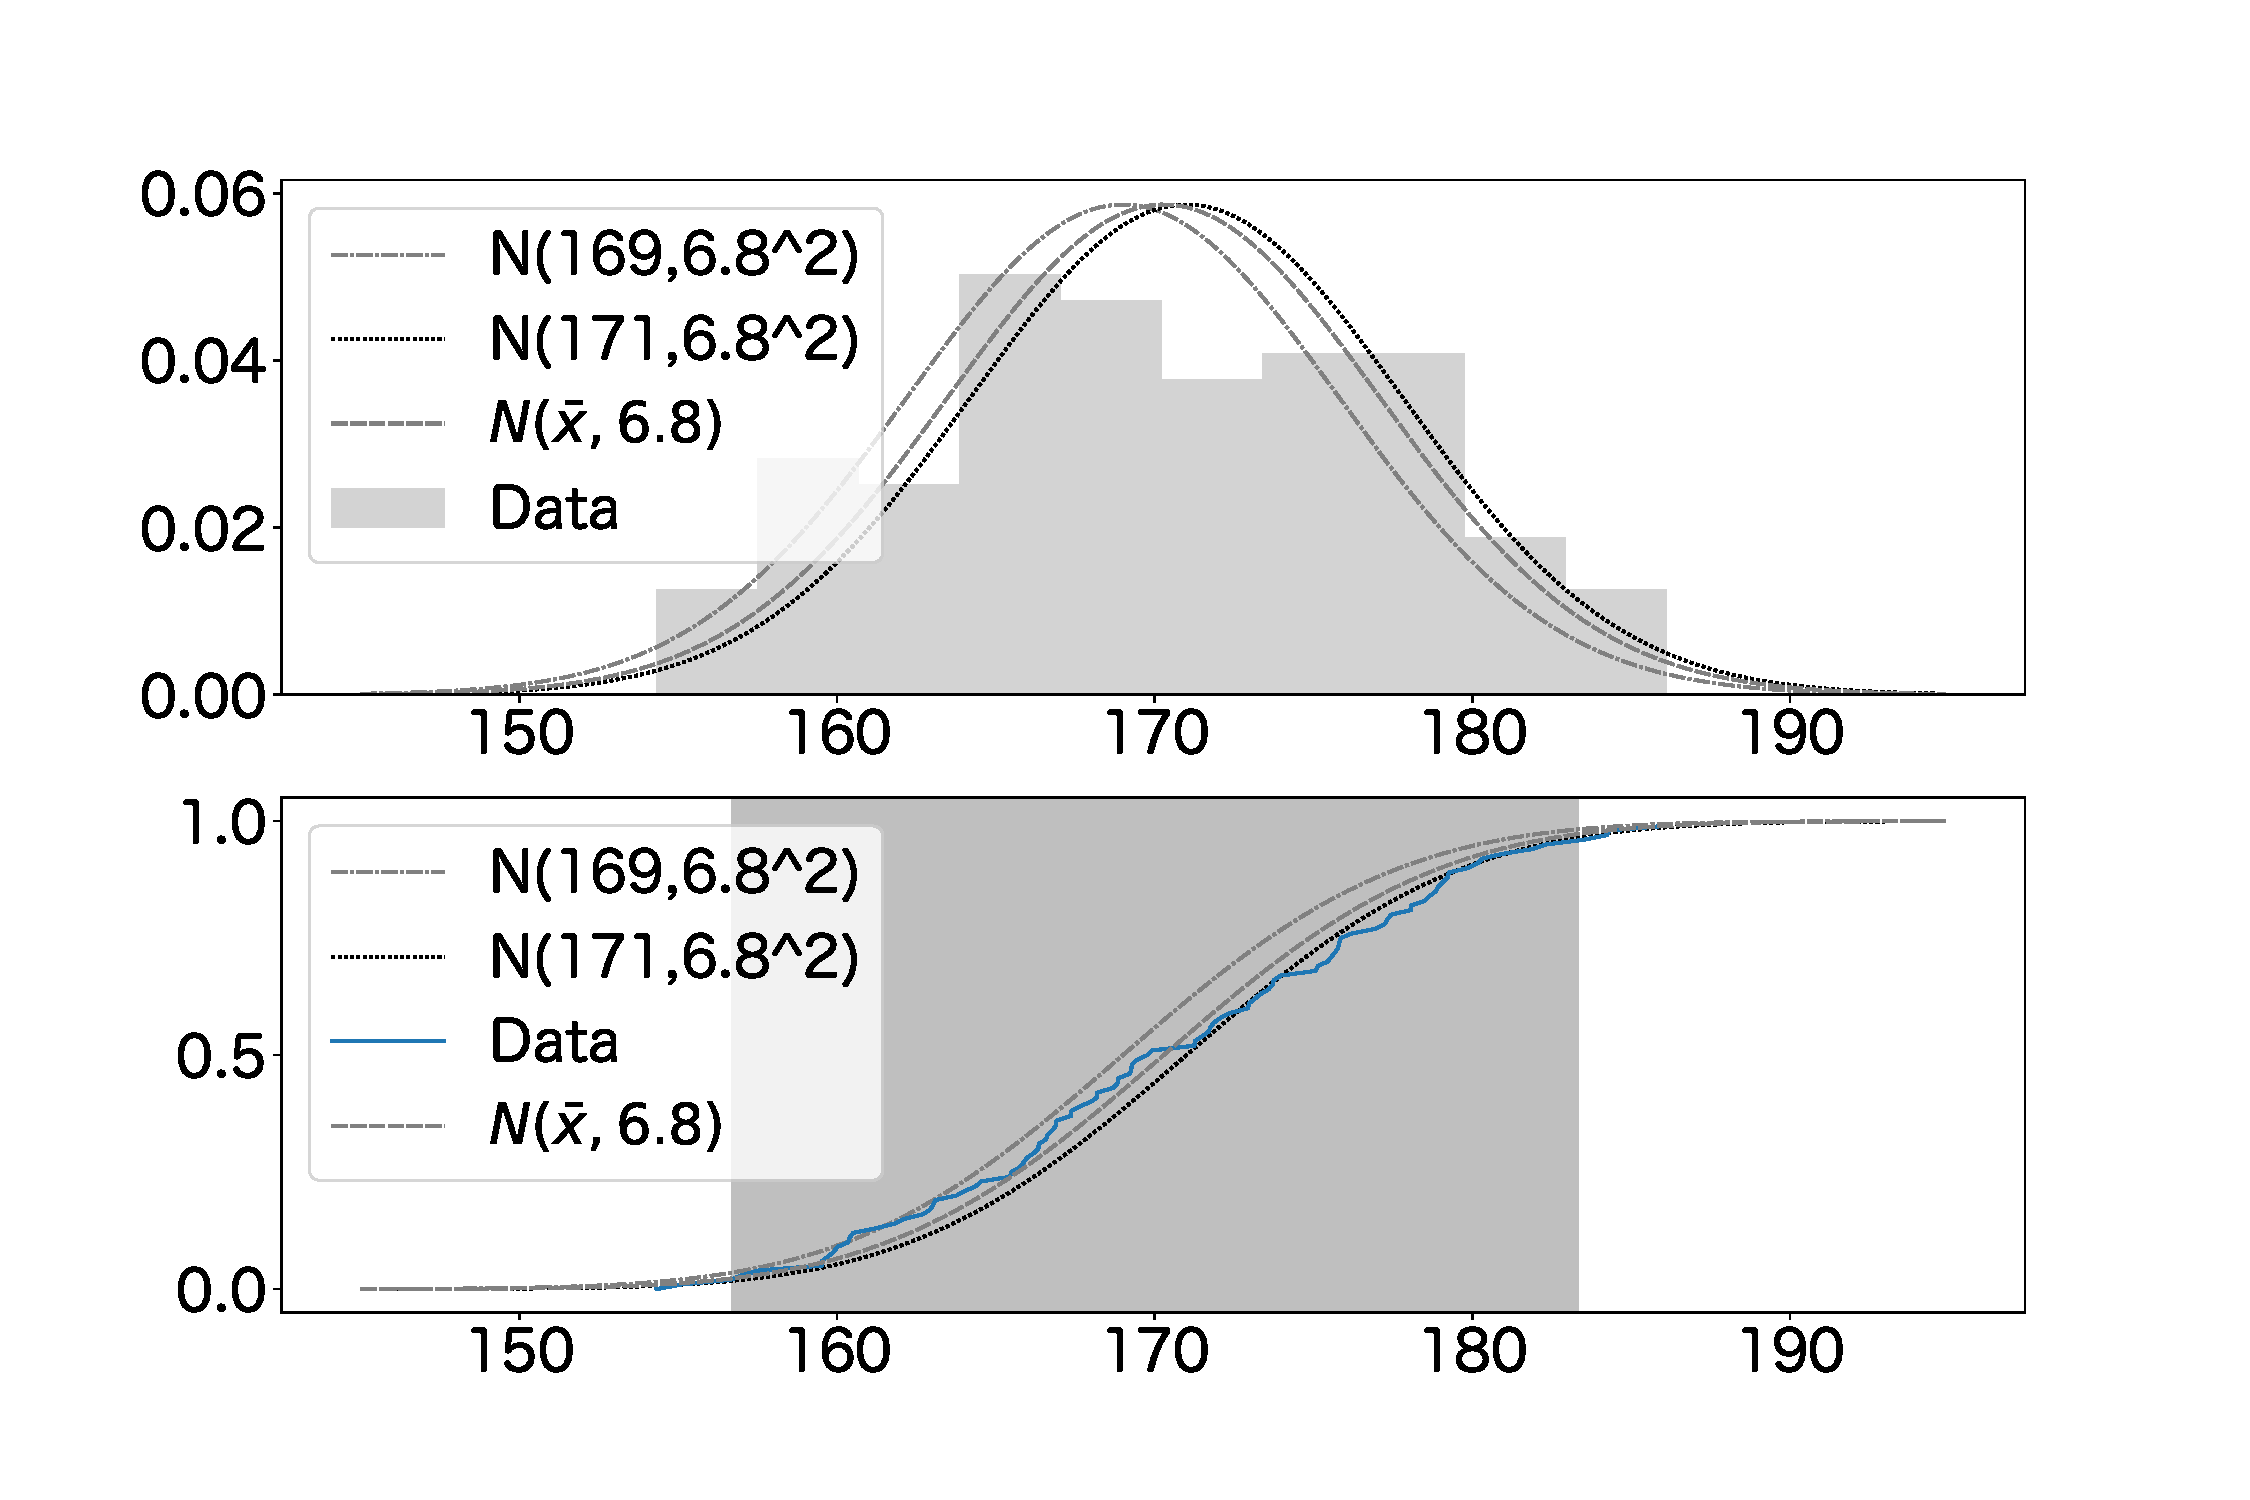
\includegraphics[width=15cm]{./image/02_/maximum_likelihood_0.pdf}
        \caption{$N(170,6.8^2)$からサンプルサイズ$100$の標本を得たときの分布。その最尤推定量により求められる分布関数。$N(168,6.8^2),N(171,6.8^2)$の分布関数を示す}
        \label{fig:maximum_likelihood_0}
    \end{center}
\end{figure}
\begin{figure}
    \begin{center}
        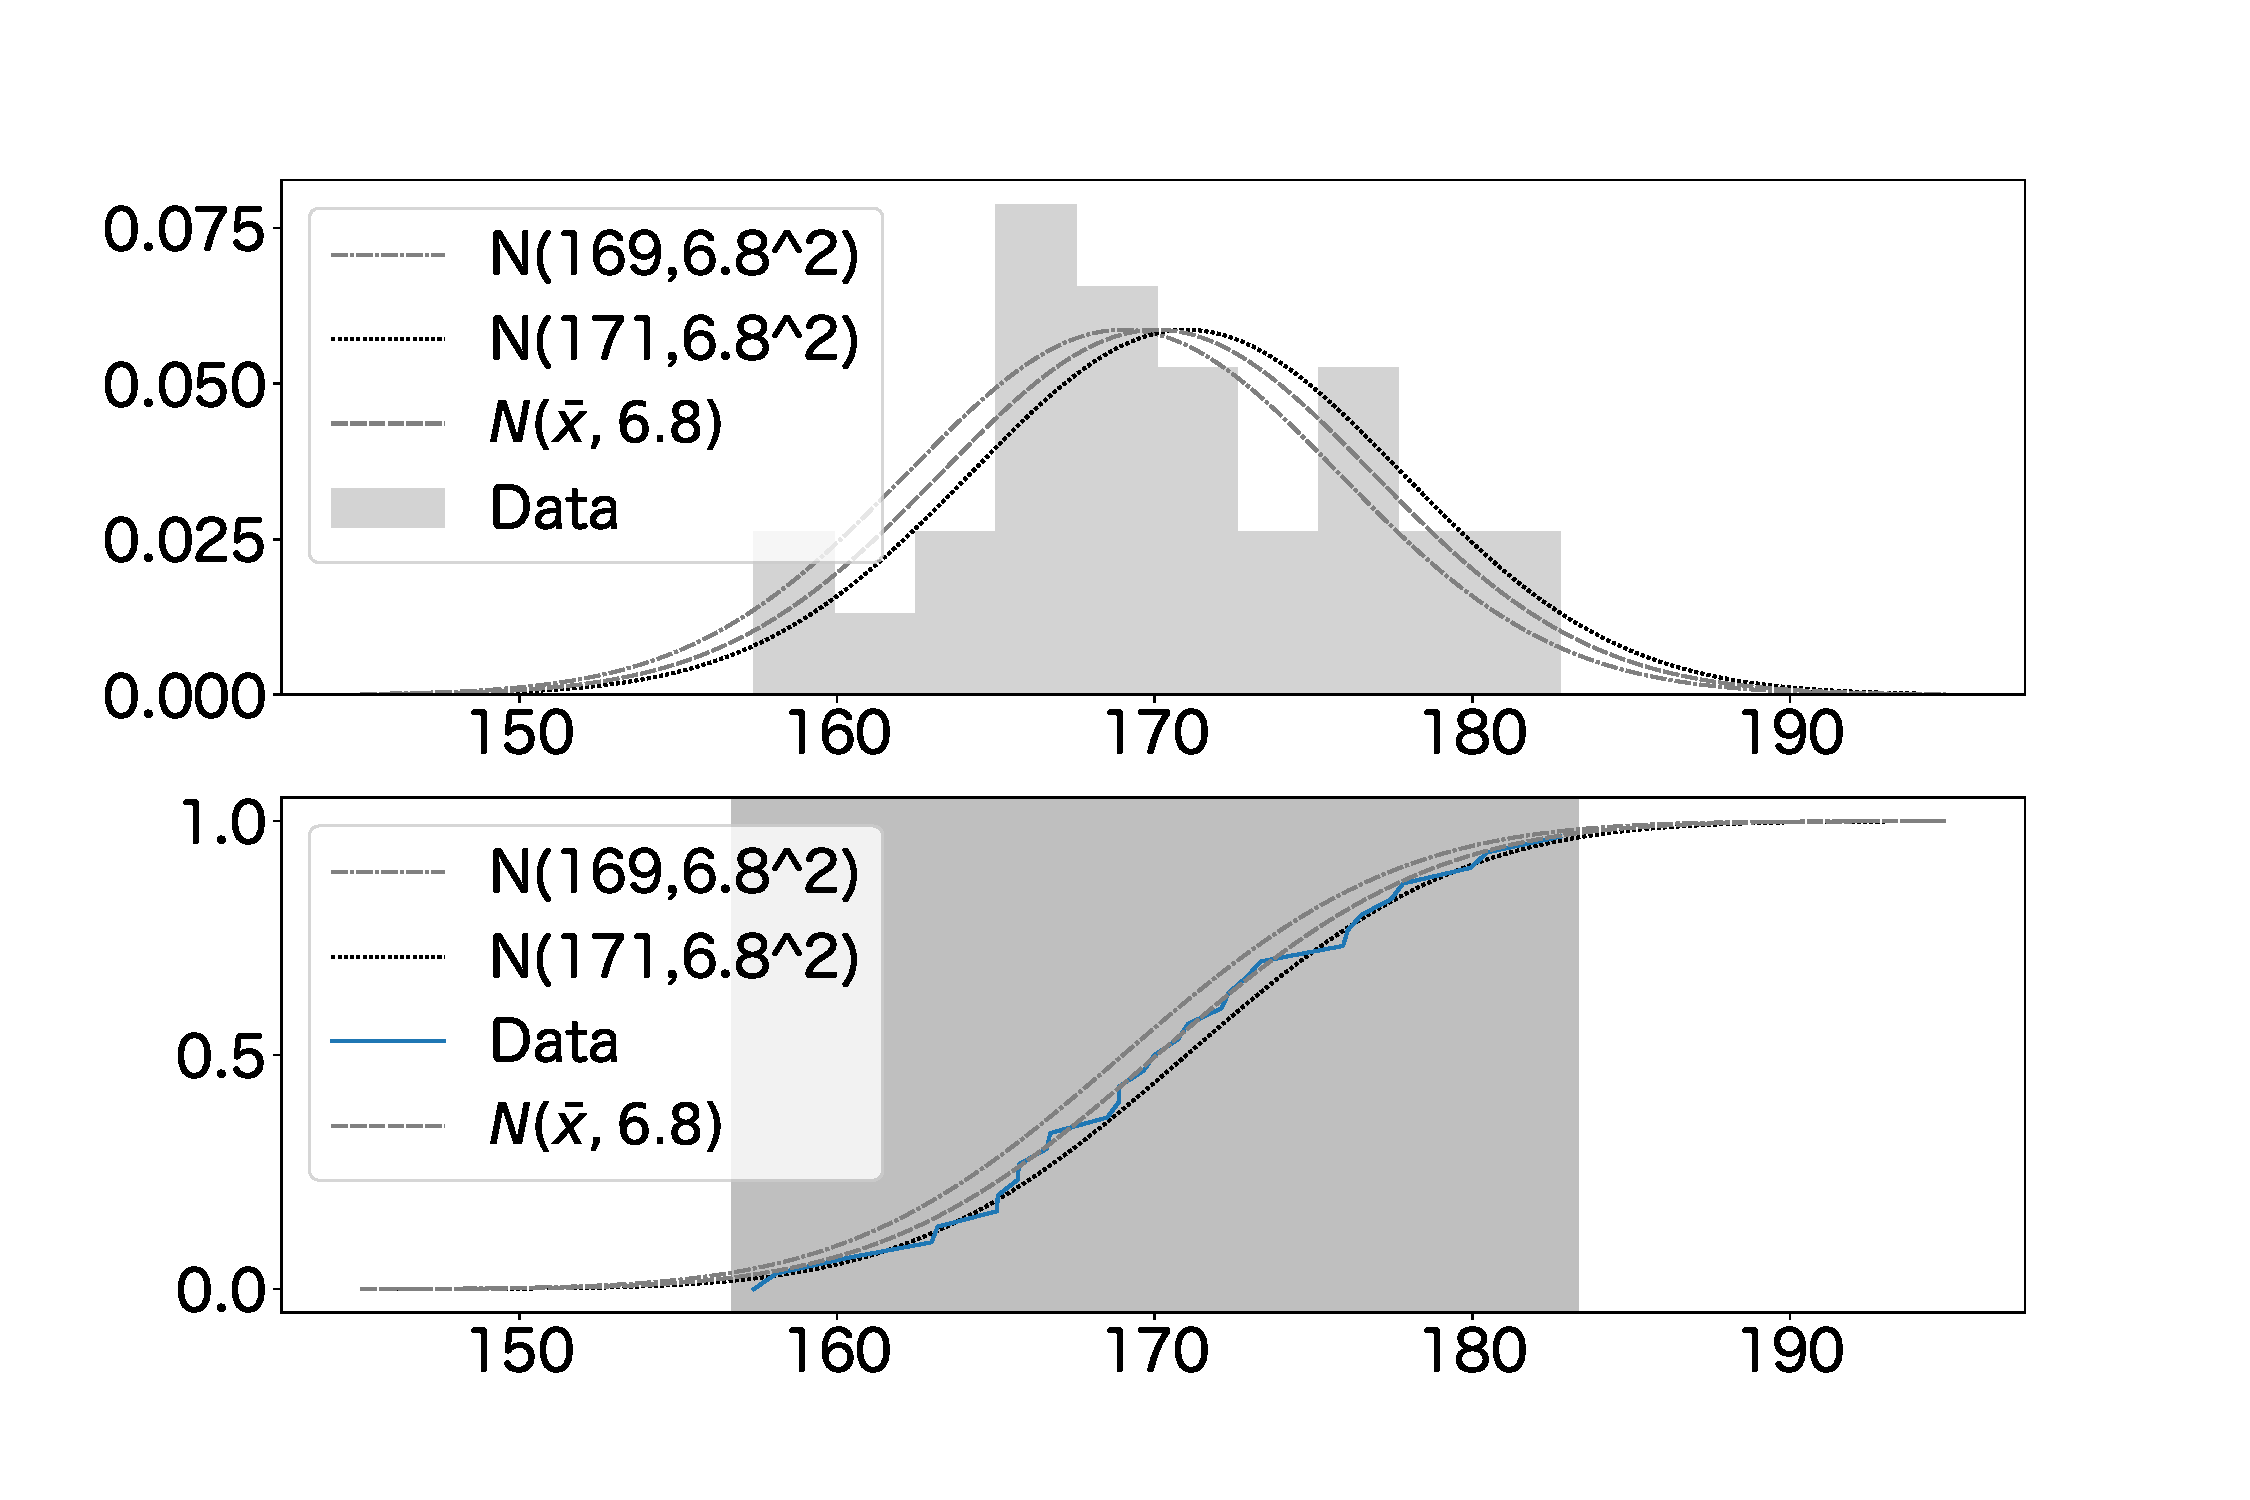
\includegraphics[width=15cm]{./image/02_/maximum_likelihood_1.pdf}
        \caption{$N(170,6.8^2)$からサンプルサイズ$30$の標本を得たときの分布。その最尤推定量により求められる分布関数。$N(168,6.8^2),N(171,6.8^2)$の分布関数を示す}
        \label{fig:maximum_likelihood_1}
    \end{center}
\end{figure}

このように、サンプルサイズが大きいと、最尤推定により推測した確率密度関数を見れば、そのほかの母数に従わないことがわかる場合がある。
また、より近くにある母数の確率密度関数と区別することは難しいこともわかる。

\begin{figure}
    \begin{center}
        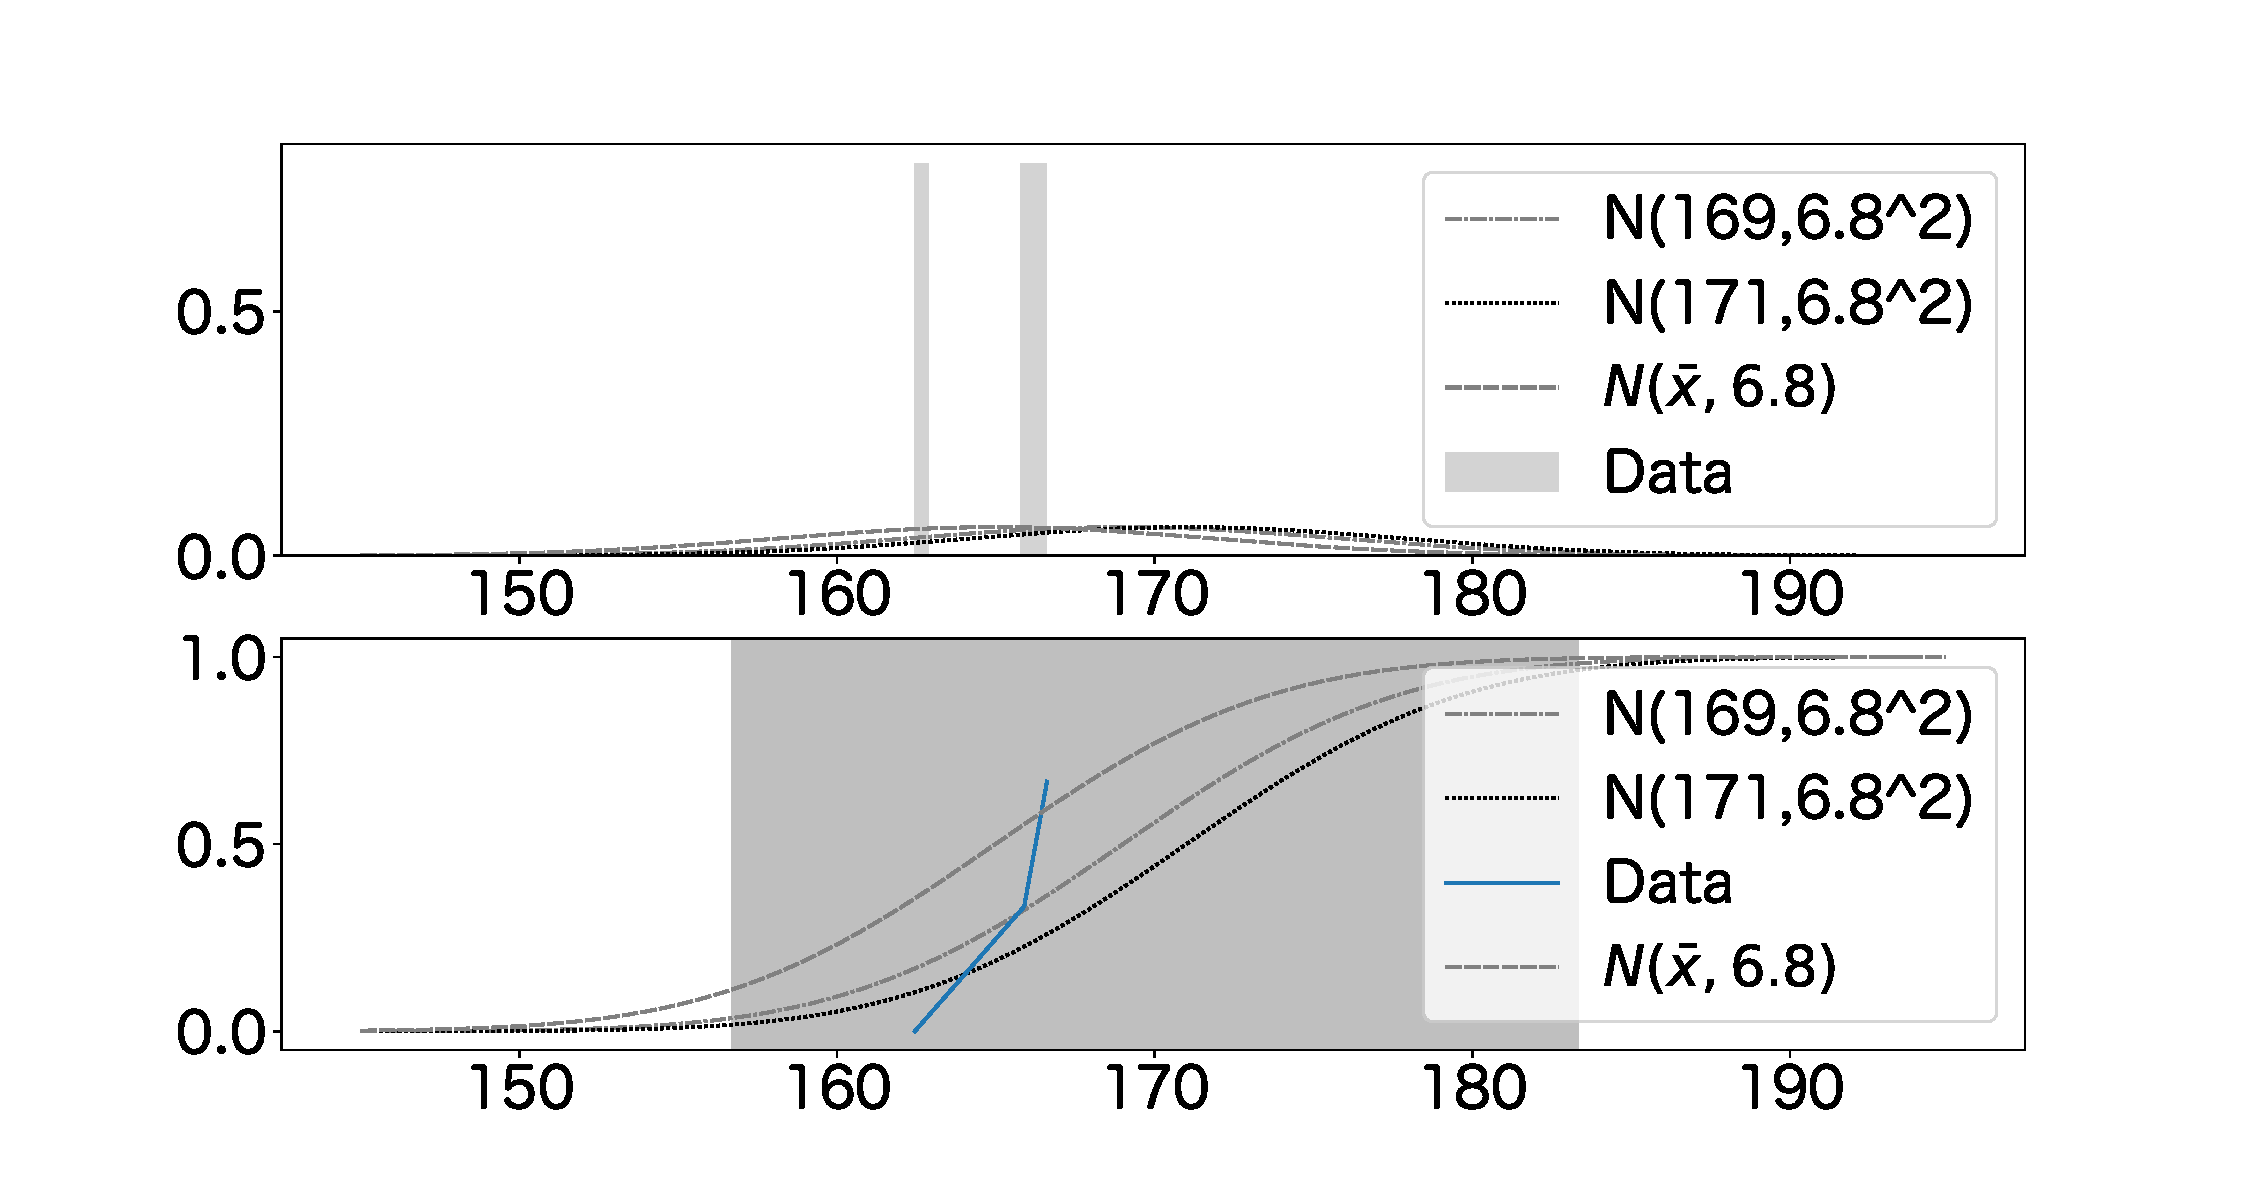
\includegraphics[width=15cm]{./image/02_/maximum_likelihood_3.pdf}
        \caption{$N(170,6.8^2)$からサンプルサイズ$3$の標本を得たときの分布。その最尤推定量により求められる分布関数。$N(168,6.8^2),N(171,6.8^2)$の分布関数を示す}
        \label{fig:maximum_likelihood_0}
    \end{center}
\end{figure}

\section{全然違うはなんとなくわかる}
図\ref{fig:maximum_likelihood_false_3},\ref{fig:maximum_likelihood_false_30}は、$N(170,6.8^2)$からサンプリングしたデータの度数分布と、その確率密度関数とは著しく異なる確率密度関数を表示したものです。

\begin{figure}
    \begin{center}
        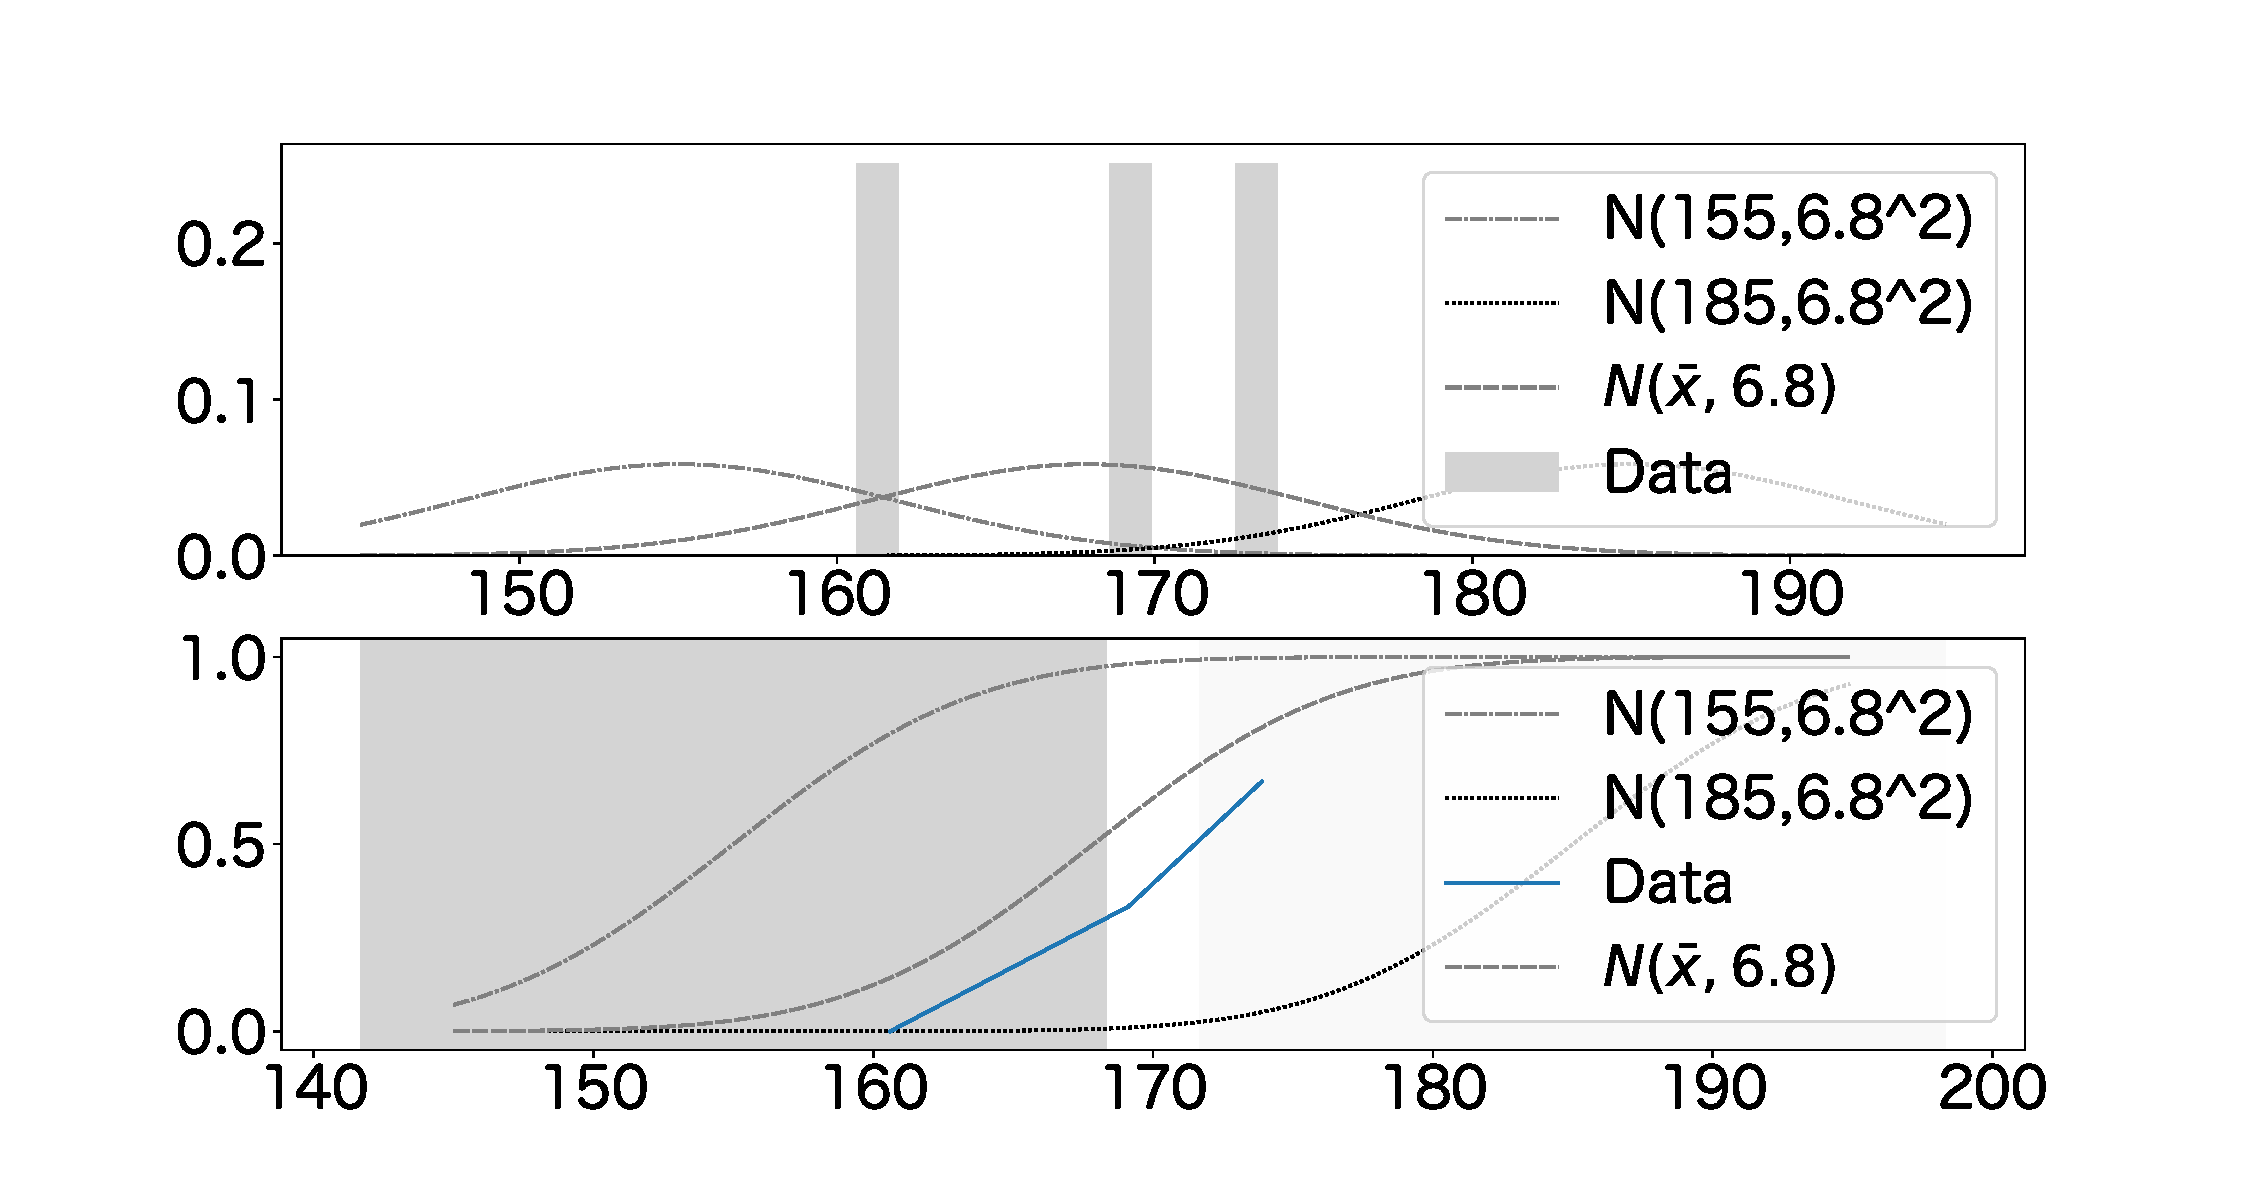
\includegraphics[width=15cm]{./image/02_/maximum_likelihood_false_3.pdf}
        \caption{$N(170,6.8^2)$からサンプルサイズ$3$の標本を得たときの分布。その最尤推定量により求められる分布関数。$N(168,6.8^2),N(171,6.8^2)$の分布関数を示す}
        \label{fig:maximum_likelihood_false_3}
    \end{center}
\end{figure}

\begin{figure}
    \begin{center}
        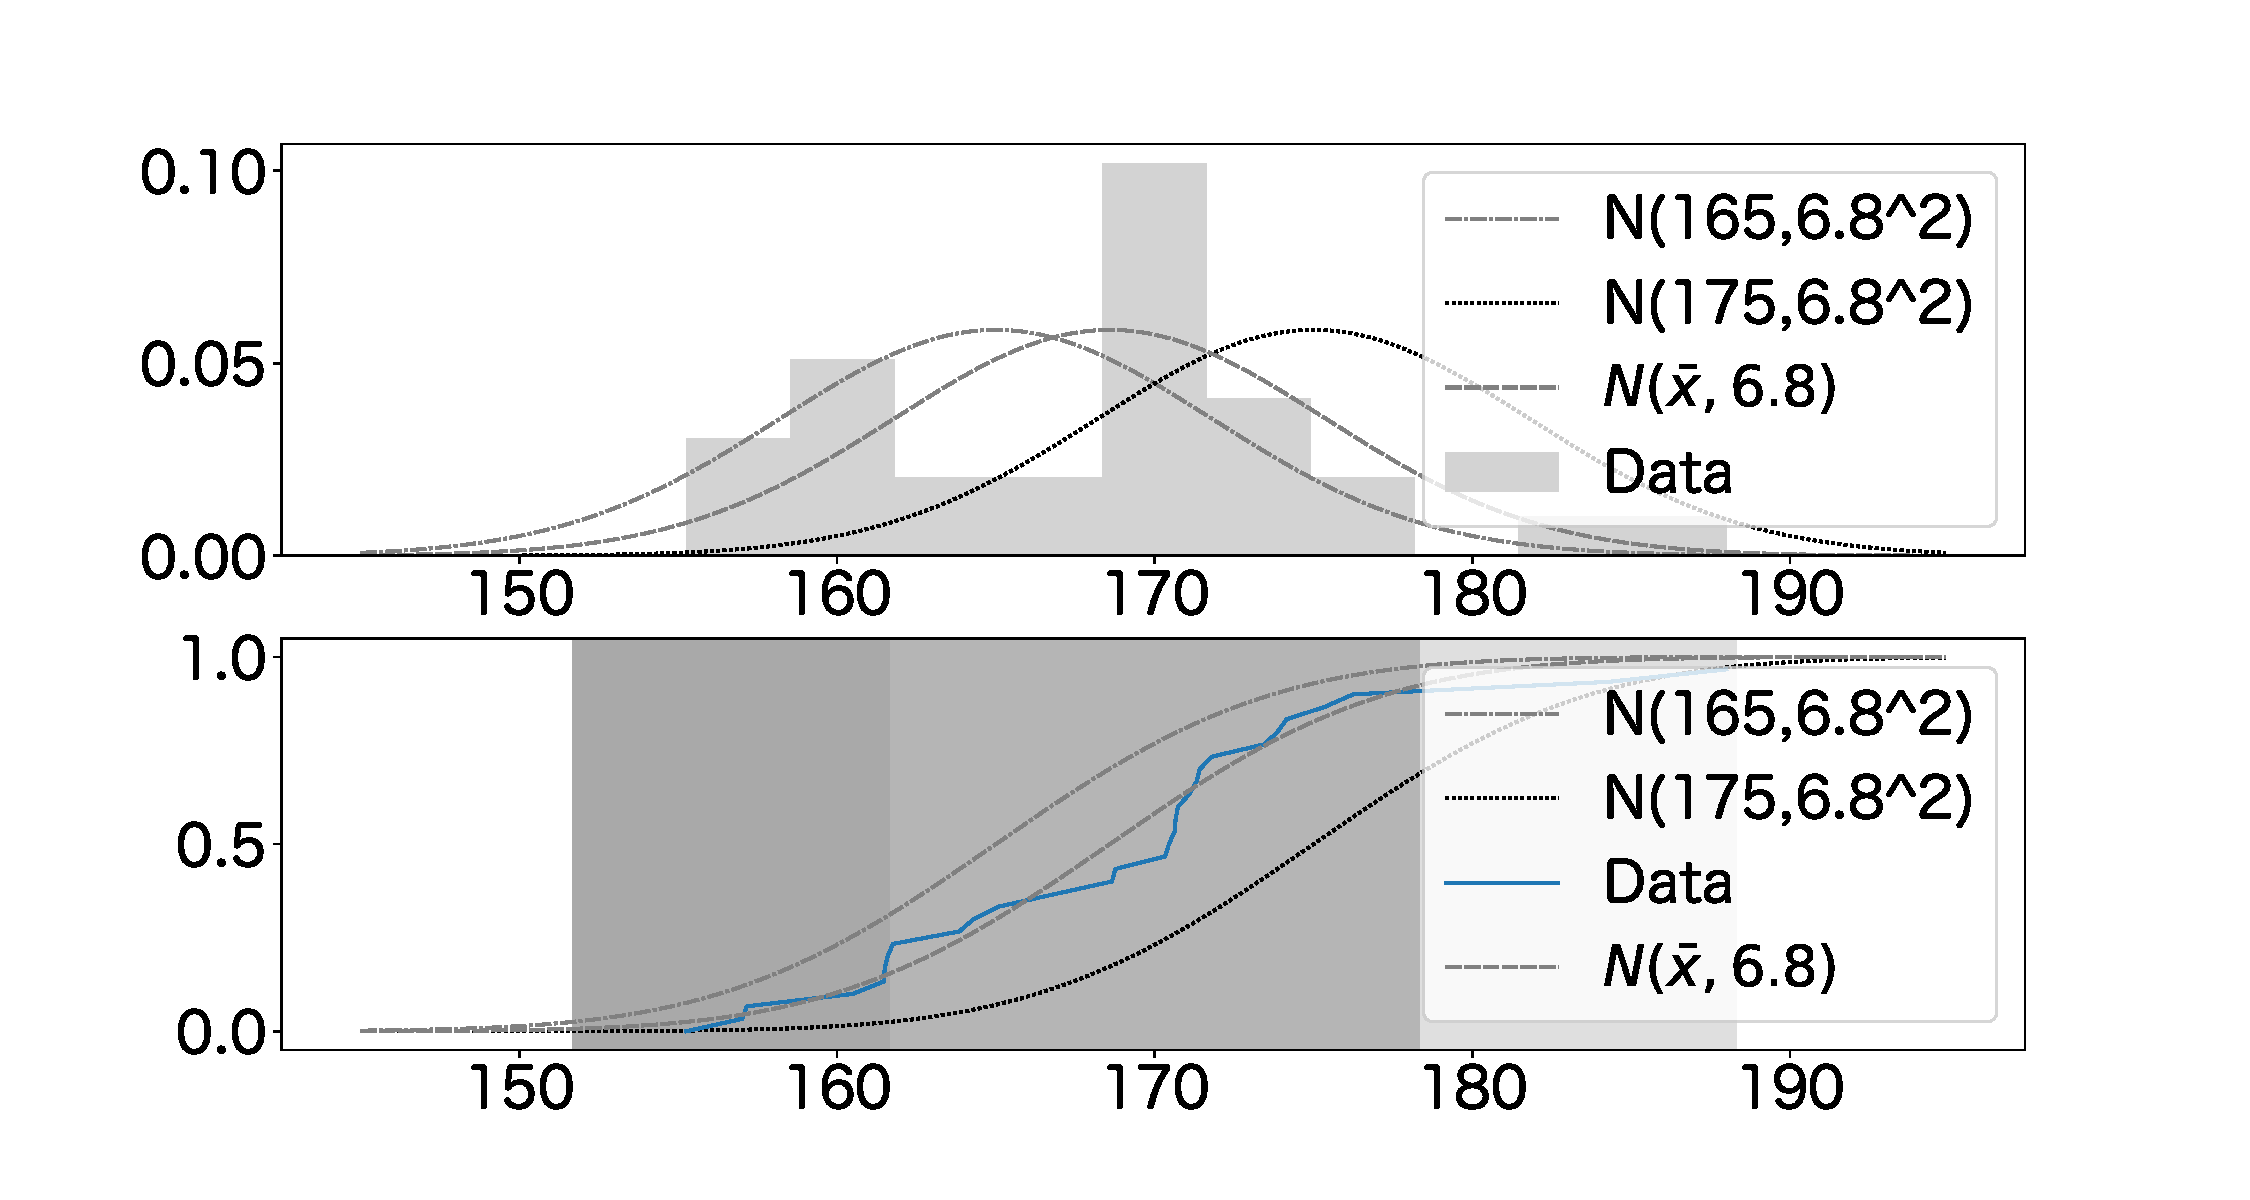
\includegraphics[width=15cm]{./image/02_/maximum_likelihood_false_30.pdf}
        \caption{$N(170,6.8^2)$からサンプルサイズ$3$の標本を得たときの分布。その最尤推定量により求められる分布関数。$N(168,6.8^2),N(171,6.8^2)$の分布関数を示す}
        \label{fig:maximum_likelihood_false_30}
    \end{center}
\end{figure}

\clearpage
\section{再生性}
\subsubsection{$(\star)$ $N(\mu,\sigma^2)$に従う確率変数であることを判定できるか}
$N(0,1)$に従う確率$x_1,x_2,\cdots,x_n$から計算した統計量、$z=\frac{\bar{X}-0}{\sqrt{\frac{1}{n}}}$は、$N(0,1)$に従い、$z$が$95\%$の確率で見つかる範囲は$[-1.96,1.96]$である。
同様に、$y_1,y_2,\cdots,y_n \sim N(1.96,1)$であるならば、$z=\frac{\bar{Y}-1.96}{\sqrt{\frac{1}{n}}}$は、$N(0,1)$に従う。

確率変数から、特定の母数を持つ正規分布に従わないことを示すことはできるだろうか。
具体的な問題設定として、
$y_1,y_2,\cdots,y_n$を正規分布に従う確率変数とする。そのとき、$y_1,y_2,\cdots,y_n$が$N(\mu,\sigma^2)$に従わないことを判断する良い方法はどのようなものだろうか。

ここで、$y_1,y_2,\cdots,y_m \sim N(1.96,1)$にもかかわらず、$N(0,1)$に従うと推測した場合、$z=\frac{\bar{Y}-0}{\frac{1}{\sqrt{n}}} \sim N(0,1)$であると考えられる。
$z$の分子の$\mu$が$0$になっていることに注意が必要である。
実際に、$y_1,y_2,\cdots y_{100}$を$N(1.96,1)$からサンプリングした標本を$100$個作ってみると、およそ$19$を中心に分布することがわかる。
このことは、$y_1,y_2,\cdots,y_m\sim N(0,1)$であるならば、$z$は、$[-1.96,1.96]$の間で$95\%$の確率で入るので、この推測が間違いであることが推測される。
以上の考察から、$y_1,y_2\cdots,y_n\sim N(0,1)$ではないと判断する。

\begin{figure}
    \begin{center}
        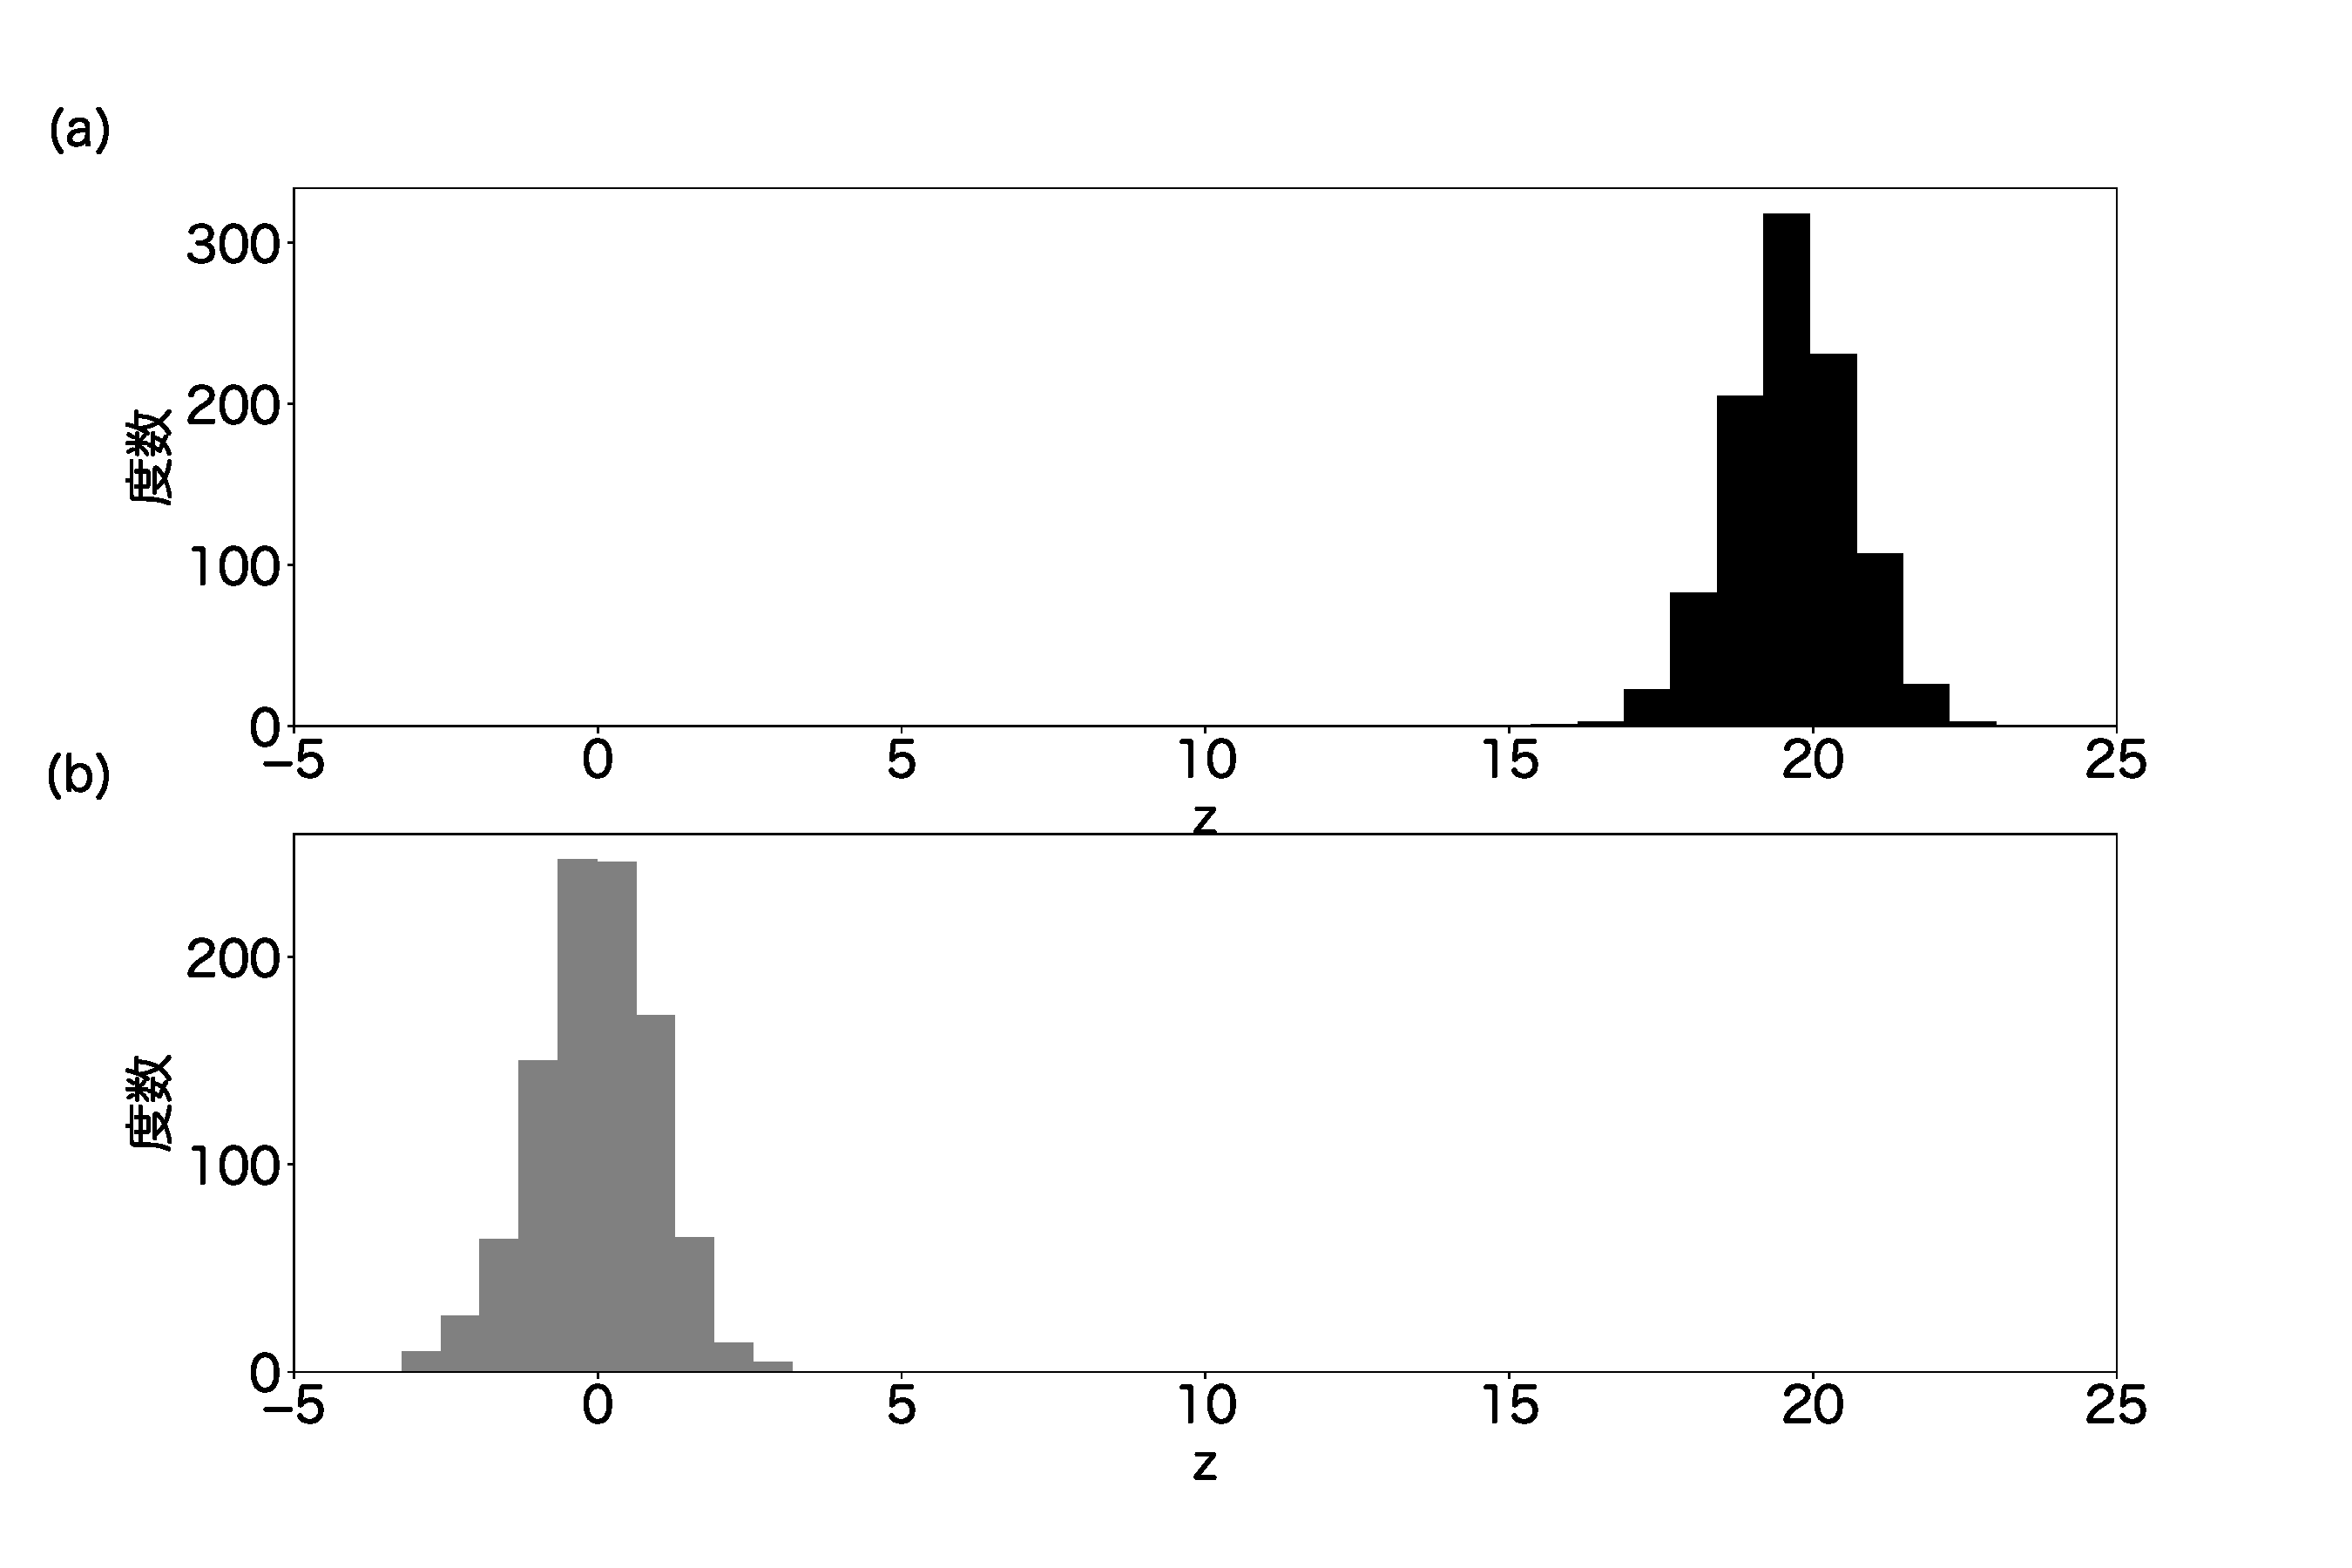
\includegraphics[width=15cm]{./image/02_/normal_distribution_test.pdf}
        \caption{(a)$N(1.96)$に従う確率変数を100個サンプリングし、その標本を1000個集めたときの$z=\sqrt{100}(\bar{X}-0)$のヒストグラム (b)$N(0,1)$に従う確率変数を100個サンプリングし、その標本を1000個集めたときの$z=\sqrt{100}(\bar{X}-0)$値のヒストグラム}
    \end{center}
\end{figure}


もう一つ例を挙げる。
$y_1,y_2,\cdots,y_n \sim N(170,5.8)$とする。このとき、この標本が$N(168,5.8)$によりサンプリングされたものではなくことを示すことはできるだろうか。
$z=\sqrt{n}\frac{\bar{y}-168}{\sigma}$を計算すればよい。
図には、$N(170,5.8)$に従う確率変数を100個サンプリングし、その標本を1000個集め、ヒストグラムを描いた。
これをみると、$0.5$を中心に分布が広がることがわかる。$z=\frac{\bar{X}-168}{\sqrt{\frac{5.8}{n}}}\sim N(0,1)$であるはずである。
複数回、標本を得た場合でも、$z$が$[-1.96,1.96]$の範囲に収まっている。このことは、$N(168,5.8)$ではないと判断できないことを示唆している。


\begin{figure}
    \begin{center}
        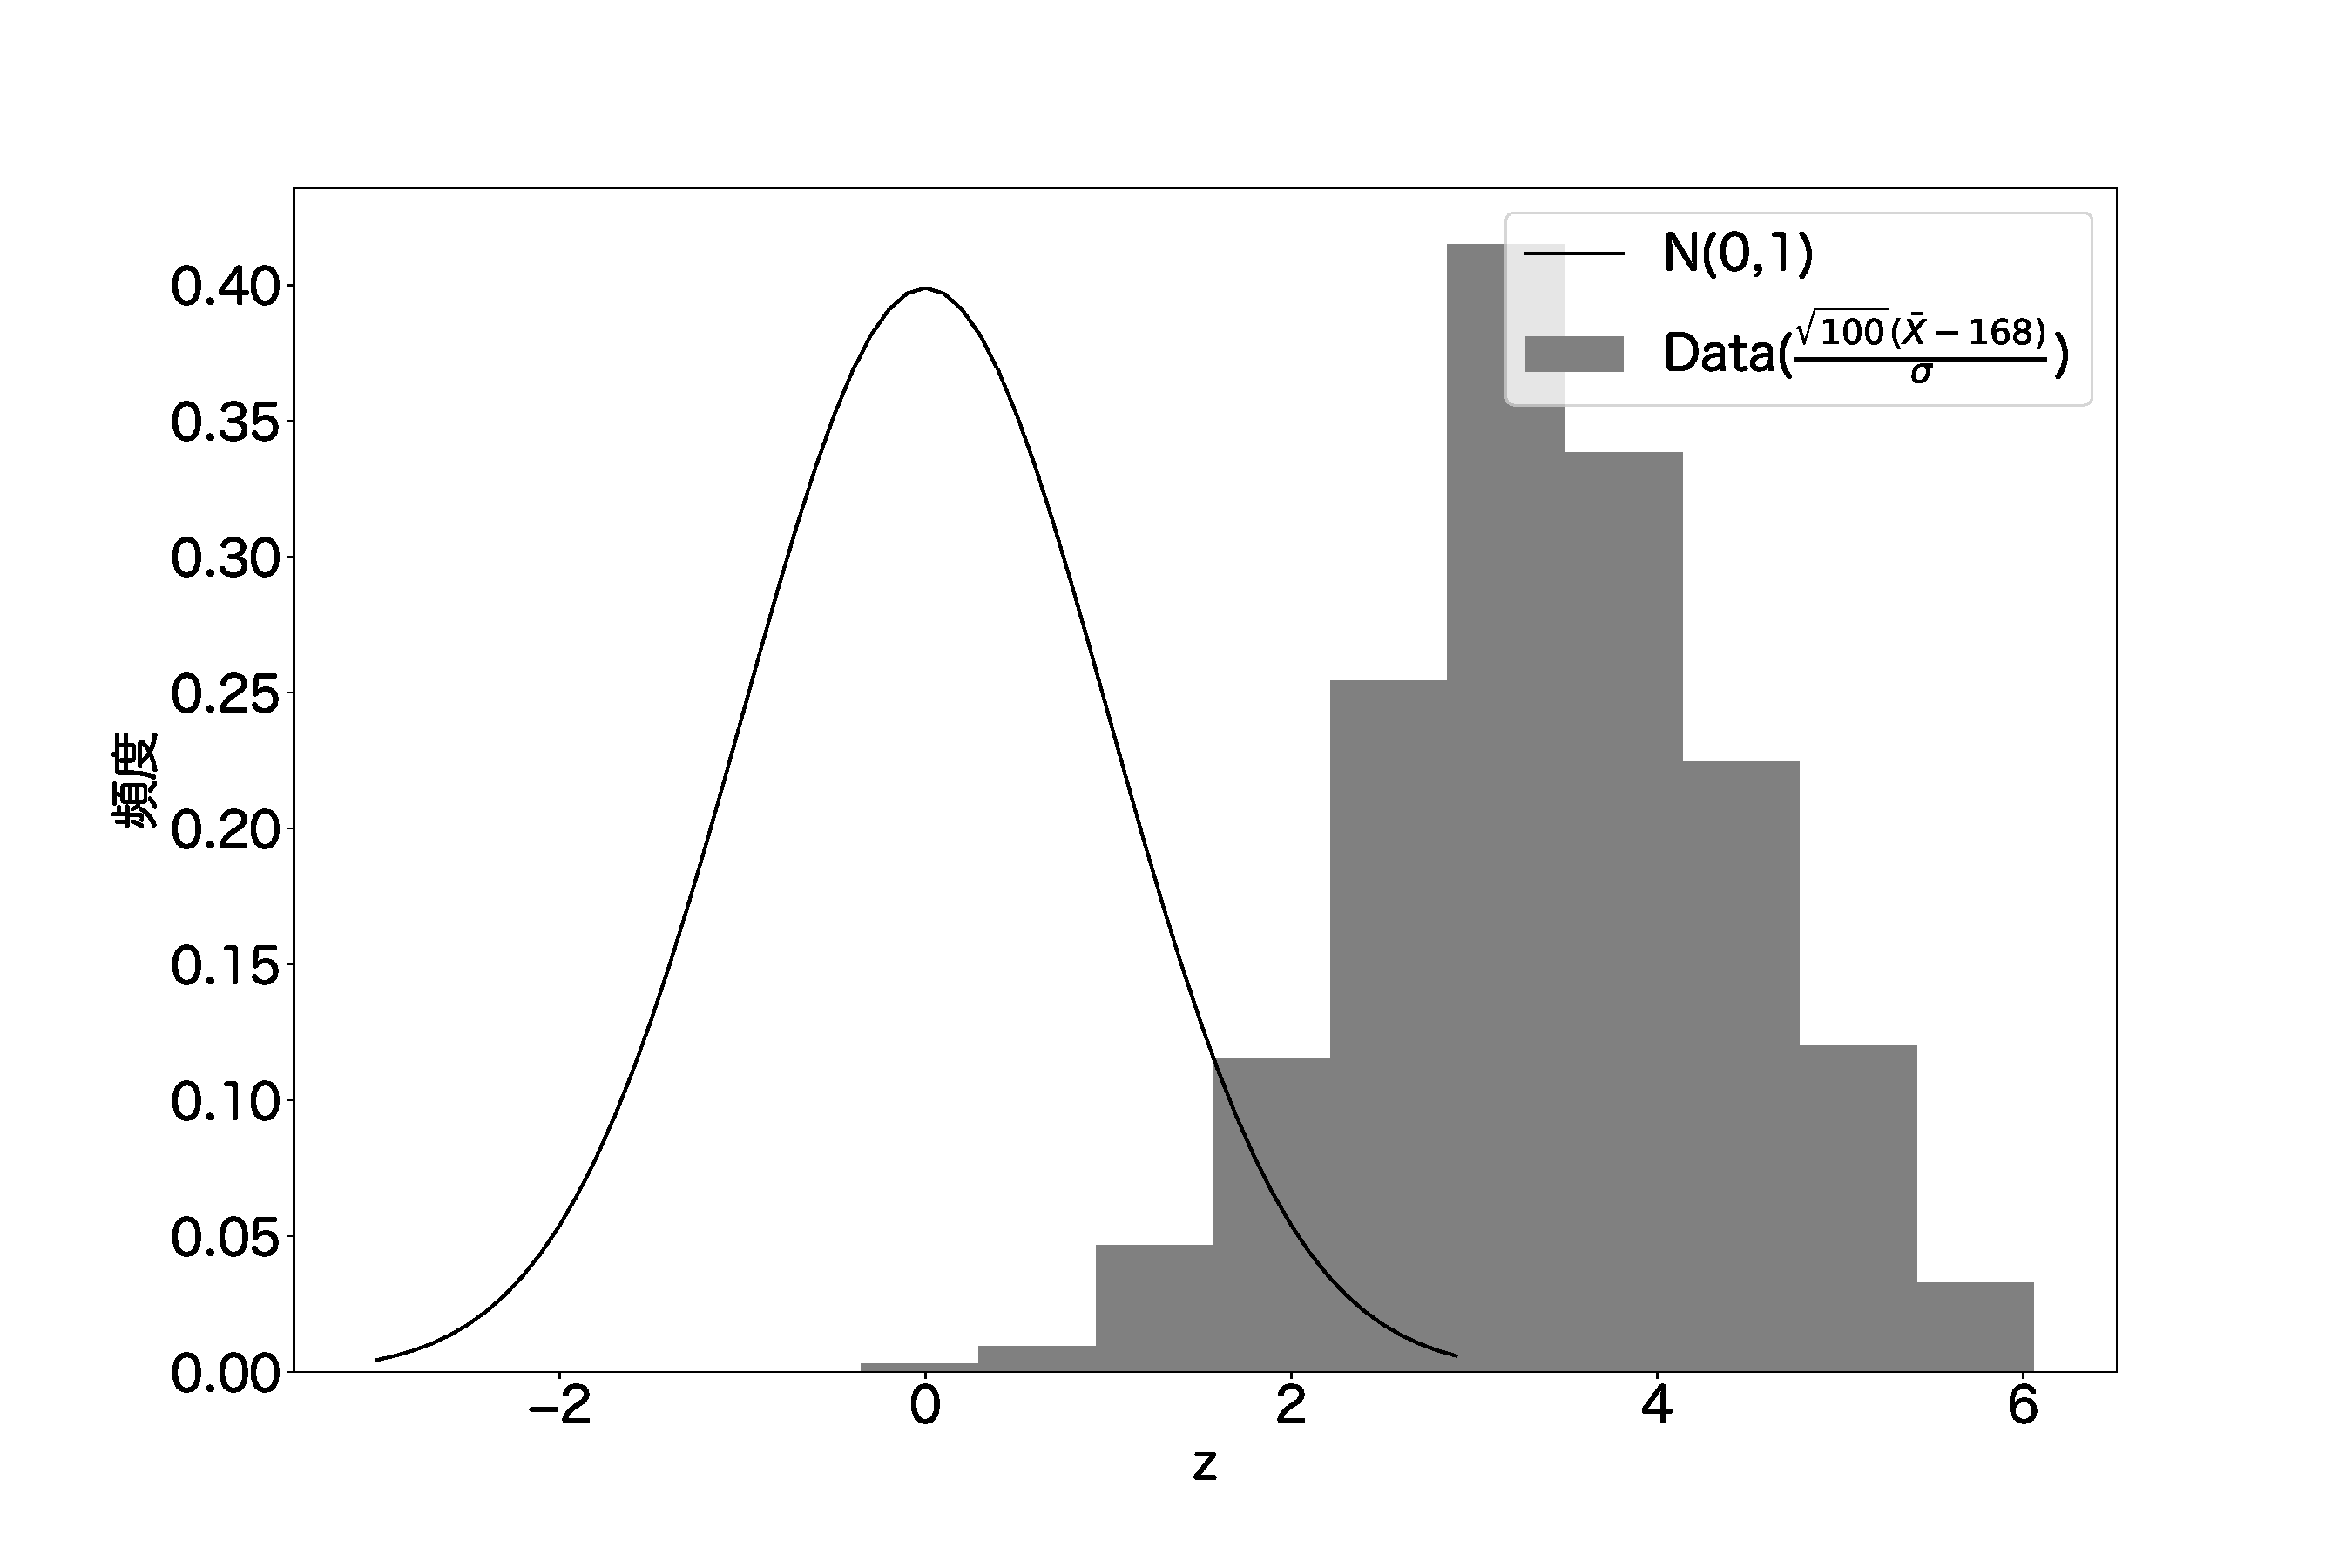
\includegraphics[width=15cm]{./image/02_/normal_distribution_test2.pdf}
        \caption{$N(170,5.8)$に従う確率変数を100個サンプリングし、その標本を1000個集めたときの$z=\sqrt{100}(\bar{X}-168)$のヒストグラム}
    \end{center}
\end{figure}


ある正規分布に従う確率変数$x_1,x_2,\cdots,x_n$が母数の異なる正規分布で得られる確率も計算できる。具体的には、$x_1,x_2,\cdots,x_n\sim N(\mu,\sigma^2)$とし、これが$N(\mu_1,\sigma_1^2)$で得られるとすると、そのときの統計量は、$z=\frac{\bar{x}-\mu_1}{\frac{\sigma_1}{n}}$である。この$z$は、$N(0,1)$に従うと考えられるので、$\phi(|z|>Z)$となる確率を計算すれば良い。

\begin{theo}
    確率変数$x_1,x_2,\cdots,x_n \sim N(\mu,\sigma^2)$ならば、$z=\frac{\bar{X}-\mu}{\sqrt{\frac{\sigma}{n}}} \sim N(0,1)$である。
    一方で、確率変数$x_1,x_2,\cdots,x_n \sim N(\mu,\sigma^2)$とする。$N(\mu_1,\sigma_1^2)$は正規分布とする。ただし、$\mu\neq \mu_1, \sigma =\sigma_1$このとき、$z=\frac{\bar{X}-\mu_1}{\sqrt{\frac{\sigma_1}{n}}} \sim N(0,1)$ではない。
\end{theo}
$\mu$と$ \mu_1$が極めて近い値のとき、$z=\frac{\bar{X}-\mu_1}{\sqrt{\frac{\sigma_1}{n}}} $も$N(0,1)$におけるよくある値になる言い換えれば、$\phi(|z|>Z)$は十分大きい。
一方で、$\mu$と$ \mu_1$が離れた値を取ると、$\phi(|z|>Z)$は小さな値になる。


\subsection{$(\star)$ $Exp(\lambda)$に従う確率変数であることを判定できるか}
$x_1,x_2,\cdots,x_n \sim Exp(\lambda)$であるとき、$n\bar{x}\sim Ga(n,\frac{1}{\lambda})$である。
母数不明の指数分布に従う確率変数が、$x_1,x_2,\cdots,x_n \sim Exp(\lambda)$と仮定したとき、$n\bar{x}\sim Ga(n,\frac{1}{\lambda})$でないならば、$x_1,x_2,\cdots,x_n \sim Exp(\lambda)$ではないと判断できるだろうか。シミュレーションによって確認してみよう。

この論法は、母数が不明の指数分布に従う確率変数を得たとき、その指数分布の母数が特定の値ではないことを示すためにこの論法を利用する。ここでは、母数が$\lambda=1,2,5,10,100$からサンプルサイズ4の標本を$1000$生成し、それら標本の統計量$n\bar{X}$のヒストグラムと、ガンマ関数$Ga(100,1)$の確率密度関数を比較する。

\begin{figure}
    \centering
    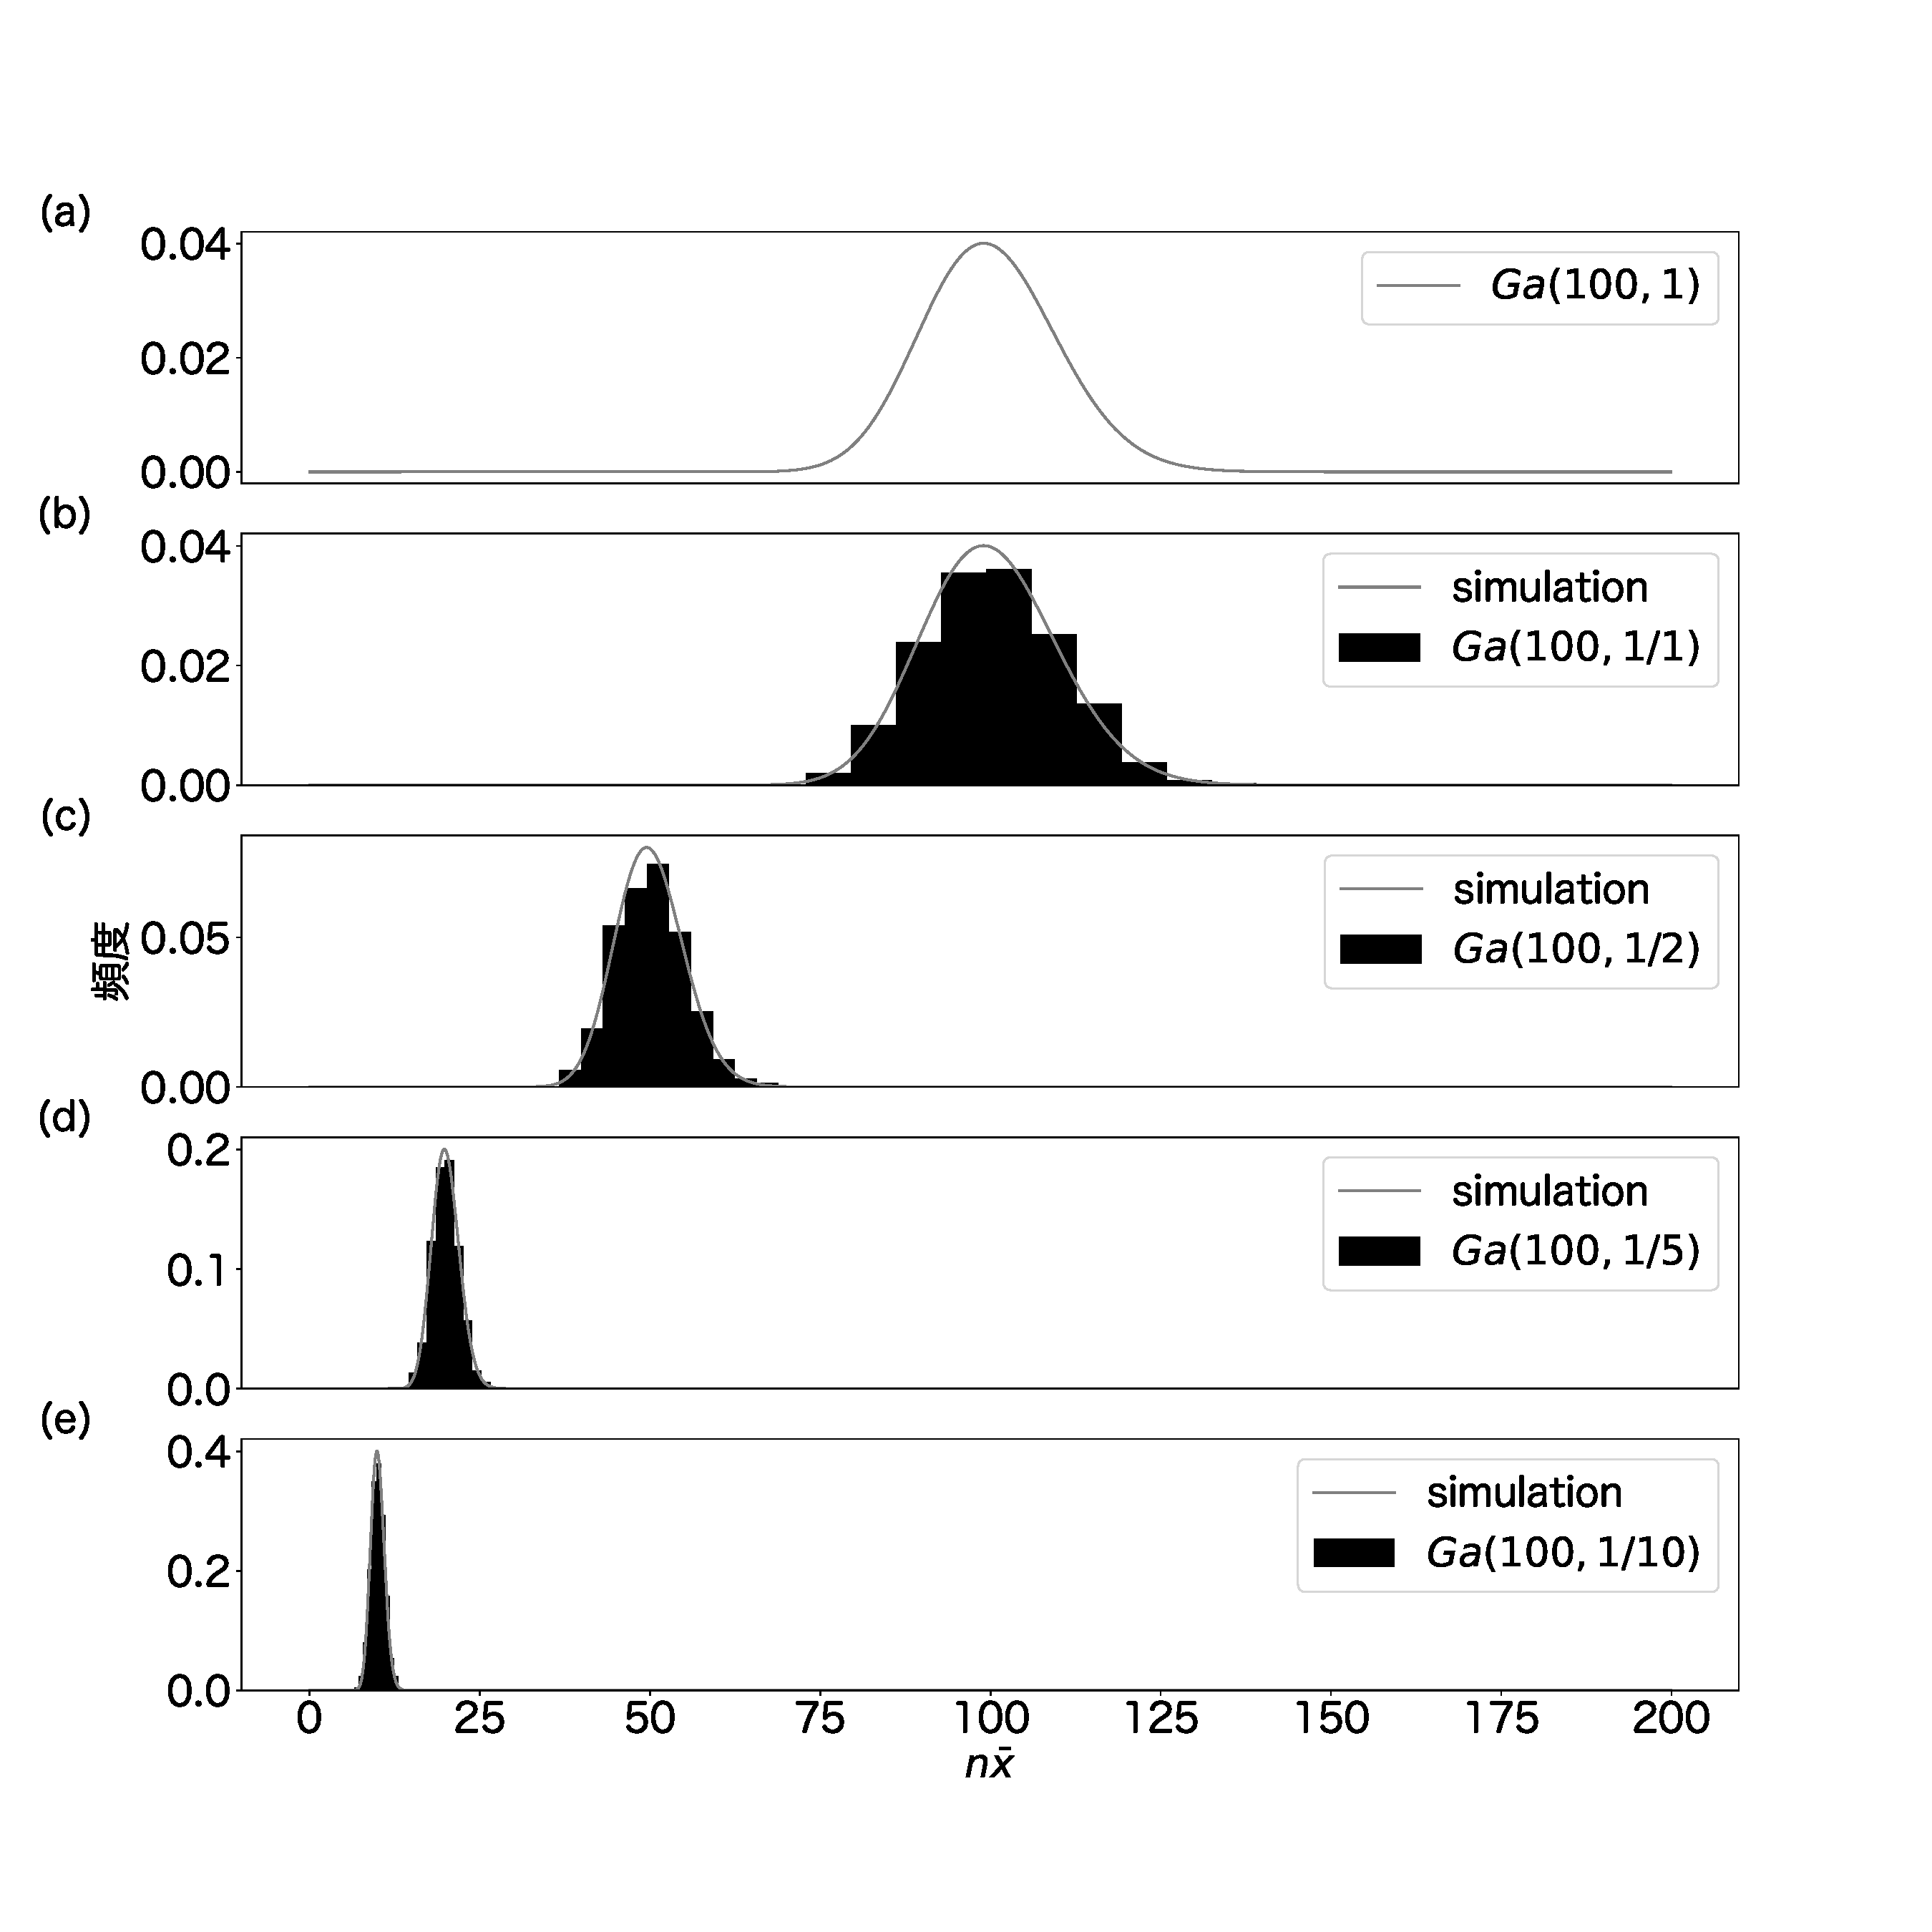
\includegraphics[width=15cm]{./image/02_/Exp_Gamma_simulation.pdf}
    \caption{(a)$Ga(10,1)$の確率密度関数。(b-e)指数分布からサンプルサイズ$4$の標本を$1000$回生成し、その統計量$n\bar{x}$のヒストグラム}
    \label{fig:exp_gamma_simulation}
\end{figure}

図\ref{fig:exp_gamma_simulation}(a)は、指数分布$Exp(\lambda=1)$の確率密度関数を示している。
図\ref{fig:exp_gamma_simulation}b-eは、シミュレーションの結果を示している。
図\ref{fig:exp_gamma_simulation}(b)には、指数分布$Exp(1)$に従う確率変数の統計量$n\bar{x}$が確かに、$Ga(100,1)$に従うことが確かめれる。
図\ref{fig:exp_gamma_simulation}(c-e)では、指数分布の$\lambda$が$1/2,1/5,1/10$のときの統計量のヒストグラムである。これらと、図\ref{fig:exp_gamma_simulation}(a)を比較すると、分布が異なっているので、確かに、$Ga(100,1)$には従わないことがわかる。



\subsection{問題点}
aa

\section{指数分布を含んだ統計モデル}
指数分布における信頼区間は式\ref{exp_model_confidence_interval}である。

\subsection{中心極限定理により信頼区間を近似する}

\section{モデルの比較}
